\RequirePackage{currfile} 
\documentclass{beamer}



%%%%%%%%%%%%%% PACKAGES %%%%%%%%%%%%%%%%%%%%%
\usepackage{textpos}   
\usepackage{graphicx} % Allows including images
\usepackage{booktabs} % Allows the use of \toprule, \midrule and \bottomrule in tables
%\usepackage{biblatex} % Allows for \cite 
\usepackage[utf8]{inputenc}
\usepackage{tikz} \usetikzlibrary{calc, arrows.meta, intersections, patterns, positioning, shapes.misc, fadings, through,decorations.pathreplacing}
\usepackage[usenames,dvipsnames]{xcolor}
\usepackage{colortbl}
\usepackage{multicol}
\usepackage{multirow}
\usepackage{caption}
%\usepackage{block} %blocks for statements
\usepackage{comment}
\usepackage[round,authoryear]{natbib}
\usepackage[absolute,overlay]{textpos}
\usepackage{array} %To hide columns
\usepackage{stix} % For arrows
\usepackage{forest}

\usepackage{array} % To hide columns
\newcolumntype{H}{>{\setbox0=\hbox\bgroup}c<{\egroup}@{}}

\forestset{qtree/.style={for tree={parent anchor=south, 
           child anchor=north,align=center,inner sep=0pt}}}



% Custom block colors for better appearance
\setbeamercolor{block title}{bg=blue!20,fg=black}
\setbeamercolor{block body}{bg=blue!10,fg=black}
\setbeamertemplate{blocks}[rounded][shadow=true]


\definecolor{ColorOne}{named}{MidnightBlue}
\definecolor{ColorTwo}{named}{Dandelion}
\definecolor{ColorThree}{named}{Plum}

\tikzstyle{descript} = [text = black,align=center, minimum height=1.8cm, align=center, outer sep=0pt,font = \footnotesize]
\tikzstyle{activity} =[align=center,outer sep=1pt]

%% Change the bg color to adjust your transition slide background color!
\definecolor{sagegreen}{RGB}{185,205,190} 
\newenvironment{transitionframe}{
  \setbeamercolor{background canvas}{bg=sagegreen}
  \begin{frame}}{
    \end{frame}
}




%%%%%%%%%%%%%% COMMANDS %%%%%%%%%%%%%%%%%%%%%
\newcommand{\progressbar}{%
\pgfmathsetmacro{\theta}{360/\inserttotalframenumber*\insertframenumber}
\begin{tikzpicture}[scale=0.025]
\fill[blue] (0,0) circle (9);
\fill[green] (0,0) -- (9,0) arc (0:-\theta:9);
\fill[white] (0,0) circle (5);
\node at (0,0) {\insertframenumber};
\end{tikzpicture}
}

%%% TIKZ STUFF
\tikzset{   
        every picture/.style={remember picture,baseline},
        every node/.style={anchor=base,align=center,outer sep=1.5pt},
        every path/.style={thick},
        }
\newcommand\marktopleft[1]{%
    \tikz[overlay,remember picture] 
        \node (marker-#1-a) at (-.3em,.3em) {};%
}
\newcommand\markbottomright[2]{%
    \tikz[overlay,remember picture] 
        \node (marker-#1-b) at (0em,0em) {};%
}
\tikzstyle{every picture}+=[remember picture] 
\tikzstyle{mybox} =[draw=black, very thick, rectangle, inner sep=10pt, inner ysep=20pt]
\tikzstyle{fancytitle} =[draw=black,fill=red, text=white]
%%%% END TIKZ STUFF

% Custom commands for colored citations
\newcommand{\citered}[1]{{\color{red}\cite{#1}}}
\newcommand{\citeblue}[1]{{\color{blue}\cite{#1}}}
\newcommand{\citesmall}[1]{{\footnotesize\cite{#1}}}
\newcommand{\citetiny}[1]{{\tiny\cite{#1}}}

% Commands for highlighting overlays
\newcommand{\highlightbox}[5]{% x, y, width, height, color
    \tikz[overlay,remember picture]{
        \draw[#5, ultra thick, rounded corners] 
        ([shift={(#1,#2)}]current page.center) rectangle 
        ([shift={(#1+#3,#2+#4)}]current page.center);
    }
}

% Most flexible version
\newcommand{\highlightboxflex}[5]{% x, y, width, height, all tikz options
    \tikz[overlay,remember picture]{
        \filldraw[ultra thick, rounded corners, #5] 
        ([shift={(#1,#2)}]current page.center) rectangle 
        ([shift={(#1+#3,#2+#4)}]current page.center);
    }
}

\newcommand{\highlightarea}[5]{% x, y, width, height, options
    \begin{tikzpicture}[overlay, remember picture]
        \draw[#5] ([xshift=#1cm,yshift=#2cm]current page.center) 
        rectangle ++(#3cm,#4cm);
    \end{tikzpicture}
}


\AtBeginSection[]{
  \begin{frame}
  \vfill
  \centering
  \begin{beamercolorbox}[sep=8pt,center,shadow=true,rounded=true]{title}
    \usebeamerfont{title}\insertsectionhead\par%
  \end{beamercolorbox}
  \vfill
  \end{frame}
}

%%%%%%%%%%%%%%% SETTINGS %%%%%%%%%%%%%%%%%%%%%%%
\mode<presentation> {
%\usetheme{Warsaw}
%\usetheme{Frankfurt}
%\usetheme{Madrid}
\usetheme{default}
%\usecolortheme{whale}
\usecolortheme{default}
\usefonttheme{professionalfonts}
}

% Bibliography setup
%\addbibresource{references.bib} % Your .bib file name
% If you prefer BibTeX instead of BibLaTeX, comment the line above and uncomment below:
\bibliographystyle{apalike}
%\bibliography{references}

%%%%%%%%%%%%%%%%%%%%%%%%%%%%%%%%%%
%FOR LINKS
\definecolor{darkblue}{rgb}{0.0, 0.0, 0.65}
\definecolor{darkgreen}{rgb}{0.0, 0.65, 0.0}
\hypersetup{
	citecolor=blue,
	colorlinks=true,
	linkcolor=blue,
	filecolor=magenta,
	urlcolor=blue
}
%%%%%%%%%%%%%%%%%%%%%%%%%%%%%%%%%%


\setbeamertemplate{navigation symbols}{} 


%Title
\title[]{When the Household Becomes the School: Sibling Effects on Parental Attention and Educational Outcomes During School Closures}
%\subtitle[]{DLP Writing Seminar}

\author[Francisco Pardo] % (optional, for multiple authors)
{Francisco Pardo - fpardo@utexas.edu \inst{1}}
 
\institute[UT] % (optional)
{
  \inst{1}%
  University of Texas at Austin
  %\and
  %\inst{2}%
   % ...
}

\date{\today}
 

 
 
%------------------------------------------------------------
%The next block of commands puts the table of contents at the 
%beginning of each section and highlights the current section:
%Commented because presentations are short, we don't need that. 
\begin{comment}
\AtBeginSection[]
{
  \begin{frame}
    \frametitle{Table of Contents}
    \tableofcontents[currentsection]
  \end{frame}
}
\end{comment}
%------------------------------------------------------------

\begin{document}


\frame{\titlepage}


\begin{frame}
    \label{frame:motivation}
    \frametitle{Motivation}

%anecdotes
%facts
%policy questions
    
    \begin{enumerate}
        \item Persistent learning losses from Covid-19 across the world, especially in more vulnerable populations. %\textcolor{blue}{cite}
        \item With school closures and kids at home, less time with teachers and peers and more with family members.
        \item Along with remote schooling, this is a drastic change in education production function.
        \item We know family size may affect children negatively when facing unexpected changes or in vulnerable populations
        %\item No evidence of the role of family size in places with significant school closures.
        
%Policy/counterfactual question:
%important deep parameter:
%Test of an important theoretical prediction:
\only<2->{
        \begin{block}{Research Question}
Do children with siblings experience larger learning losses when households face an unexpected shock/school closures/increased childcare needs?
\end{block}
}
    \end{enumerate}
    
\end{frame}





%Just enough of your methodology so results don't feel like magic
%Not so much that you crowd out the ndings
\begin{transitionframe}
    \label{frame:thispaper}
    \frametitle{This Paper}
    \begin{enumerate}
    \item I use a DID strategy to compare children with siblings with only children before and after school closures.
    \item Both populations had equal trends before the pandemic
    \item I find students with siblings do 0.06sd worse in GPA and 0.1 in standardized scores. 
    %\item parents reduced expectations in XX
    \item Mechanisms
    \item External validity
    \end{enumerate}
\end{transitionframe}

\begin{frame}
    \label{frame:contribution}
    \hypersetup{citecolor=blue}
    \frametitle{Contribution to literature}
    \begin{enumerate}

    \item \textbf{Quantity-Quality:} Most papers find no reductions in quality of education when family size increases. {\footnotesize\cite{becker_child_1976}, \cite{black_more_2005}, \cite{caceres-delpiano_impacts_2006} \cite{conley_parental_2006}}. There might be if unexpected or vulnerable. {\footnotesize\cite{black_small_2010}, \cite{aslund_family_2010}.}
    $\rightarrow$ I find that the influence of family size may depend on how much the family is pushed towards constraints.

    \item \textbf{Health Shocks:} {\footnotesize\cite{adhvaryu_endowments_2016}}

    \item \textbf{School closures:} 
    {\footnotesize \cite{haelermans_inequality_2022}, \cite{jakubowski_global_2023}}
   
    
     
        %\item \textbf{Covid Learning Loss} \\
        %\item \textbf{Universal Pre-K}: Is there a sibling spillover effect in this space due to released time? I see new literature like Jackson et al (2025), Humphries et al (2025) mostly on increased labor/earnings.
        %\item \textbf{Health Shocks}: 
        %\begin{itemize}
        %    \item Siblings with disabilities: Black et a
        %\end{itemize}
        %\item \textbf{Parental Investment} \\
        %\item \textbf{Quanity-Quality} \\
        %\item \textbf{Universal PreK:} \\
        %$\uparrow$ labor and earnings. Benefits $>>>$ Costs. \\
        %\small \textcolor{gray}{Jackson, Turner, Bastian (2025), Humphries et al (2025)}

    \end{enumerate}
\end{frame}

\begin{transitionframe}
    \label{frame:background}
    \frametitle{Background and Context}
    \begin{enumerate}
       \item Covid in Peru
       \item School closures in Peru
       \item What does this mean?
       \item How much more were parents involved?
       \item What happened to performance?
    \end{enumerate}
\end{transitionframe}

% ========================================
% DATA
% ========================================
\begin{frame}
    \label{frame:data}
    \frametitle{Data}

    \begin{itemize}
        \item School progression (approval and GPA per grade-year)
        \item Standardized test scores in 2nd, 4th, 6th, 8th grade in some years.
        \item Family, student, teachers and principals surveys:
        \begin{itemize}
            \item Parental involvement in children's education
            \item Socioeconomic Status
            \item Aspirations for higher education: parents (2nd and 4th grade) and students (8th grade)
            %\item Gender beliefs: "Boys are better at Math than girls"
            %\item Parental involvement: my parents ask me about my grades, I talk to my parents about what I read, why they chose school, gender beliefs, overall knowledge about school/child, etc
            %\item studying habits, beliefs, etc
            %\item Specifically related to siblings: ``Read out loud to my siblings''.
        \end{itemize}
        \item Identify siblings through parent's anonymized ID.
    \end{itemize}
\end{frame}

% ========================================
% DATA
% ========================================
\begin{transitionframe}
    \label{frame:trends}
    \frametitle{Trends in data}
    \begin{columns}[T]
        \begin{column}{0.48\textwidth}
            \centering
            \textbf{\% of A's in Mathematics}
            \vspace{0.2cm}
            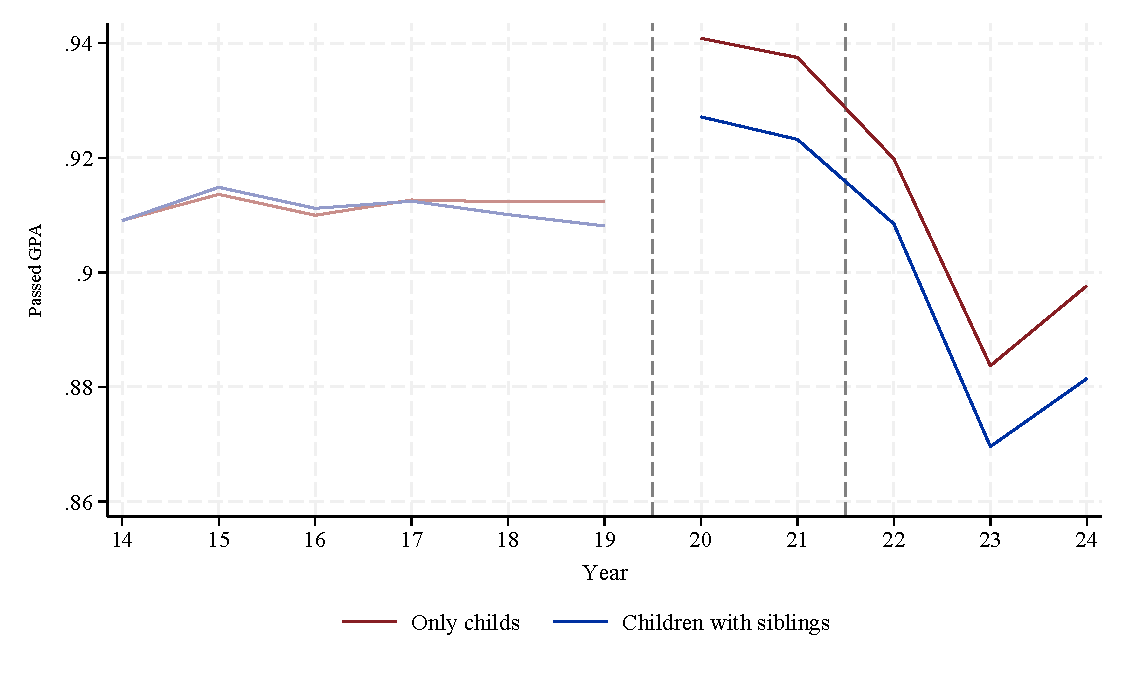
\includegraphics[width=\textwidth]{./FIGURES/Descriptive/raw_total_elm_pass_math_siblings.pdf}
        \end{column}
        \begin{column}{0.48\textwidth}
            \centering
            \textbf{Standardized GPA in Mathematics}
            \vspace{0.2cm}
            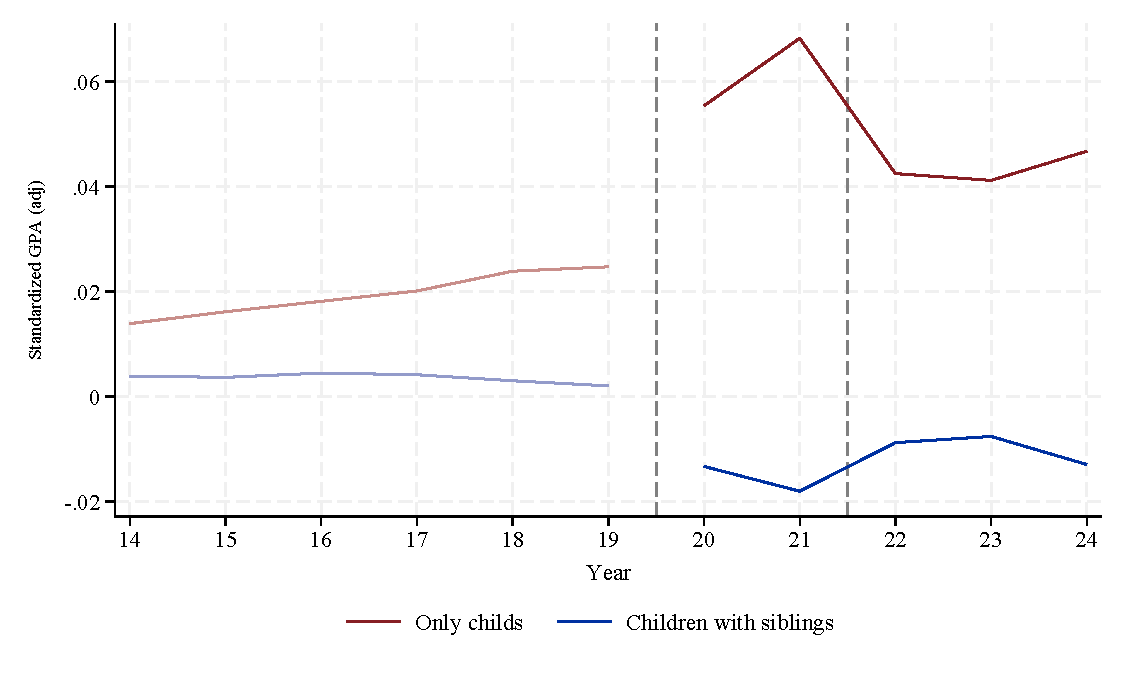
\includegraphics[width=\textwidth]{./FIGURES/Descriptive/raw_total_elm_std_gpa_m_adj_siblings.pdf}
        \end{column}
    \end{columns}
    
    
\end{transitionframe}

% ========================================
% RESEARCH
% ========================================
\begin{frame}
    \label{frame:research}
    \frametitle{Research Design}
    
    \begin{block}{Identification Strategy}
    Differential changes between only children and children with siblings before and after the pandemic.
    \end{block}
    
    \begin{itemize}
         \item<2-> \textbf{No anticipation:} Given the unexpected nature of the pandemic, families couldn't have chosen to have or not have children or be affected by school closures before they happened. \\
         $\Rightarrow$ School closures were unexpected, especially if thinking about fertility
         \item<3-> \textbf{No unobserved time varying shocks:} For example, if one parent doesn't work they may choose to have more children but also have more time for homeschooling (\textcolor{blue}{+}) or may need children to work (\textcolor{red}{-}). \\
         $\Rightarrow$ Strategy controls for any unobserved time invariant shock. However, will provide some evidence with IV estimates.
    \end{itemize}

\end{frame}


% ========================================
% EMPIRICAL STRATEGY
% ========================================
\begin{frame}
    \label{frame:empirical}
    \frametitle{Empirical Strategy}

    
    \textbf{Difference-in-Differences Specification:}
    \small
    \begin{align}
    Y_{ist} &= \alpha + \delta_1 \text{Post}_{it} + \delta_2 \text{HasSiblings}_{i} \nonumber  \\
    &\quad + \boldsymbol{\beta} (\text{Post}_{it} \times \text{HasSiblings}_{i}) \nonumber \\
    &\quad + \mathbf{X}_{ist}'\gamma + \lambda_s + \mu_t + \varepsilon_{ist}
    \end{align}
    
    \vspace{0.1cm}
    
    \textbf{Event Study Specification:}
    \begin{align}
    Y_{ist} &= \alpha + \sum_{k=-5}^{-2} \delta_k (\mathbb{I}[t = 2020+k] \times \text{HasSiblings}_{i}) \nonumber \\
    & \quad + \sum_{k=0}^{4} \beta_k (\mathbb{I}[t = 2020 + k] \times \text{HasSiblings}_{i}) \nonumber \\
    & \quad + \mathbf{X}_{ist}'\gamma + \text{HasSiblings}_{i} + \lambda_s + \mu_t + \varepsilon_{ist}
    \end{align}
    \normalsize
    
    %where $\tau_d$ is the treatment date for district $d$, and we normalize $\beta_{-1} = \delta_{-1} = 0$.
    
\end{frame}


% ========================================
% RESULTS
% ========================================


% A, Main Results

%A.1. Event Study (all siblings)
    %covid_event_all_all_std_gpa_m_adj_Tsiblings_Sall_4
    
%A.2. Event Study (by siblings)
    %covid_event_bysibs_all_all_std_gpa_m_adj_Tsiblings_Sall_4

% B. Mechanisms
%B.1. Birth Order
%% Double sided event and GPA bar

%B.2. Sibling rivalry
%2.1 Bar GPA by PC/internet

%2.2 Bar GPA by Age gap

%B.3. Parental time
%3.1. Descriptives about parent's
    %Who spends more time with their kids.
%3.1. By parent's

%B.4 Income
%Change in SES
%twfe_ses_2_4_8_Tsiblings_Soldest_4

% C. Other Outcomes
%C.1. Results by grade 2/4/6/8 GPA (TWFE bar plots)
    %twfe_gpa_2_4_6_8_20_21_Tsiblings_Soldest_4

%C.2. Results by grade 2/4/8 ECE
    %twfe_ece_2_4_8__Tsiblings_Sall_4

%C.3. Grade promotion
    
%C.4. College application

\begin{frame}
    \label{frame:eventstudy}
    \frametitle{Children with siblings do compared to only children during school closures}
        {\resizebox{0.9\textwidth}{!}{
       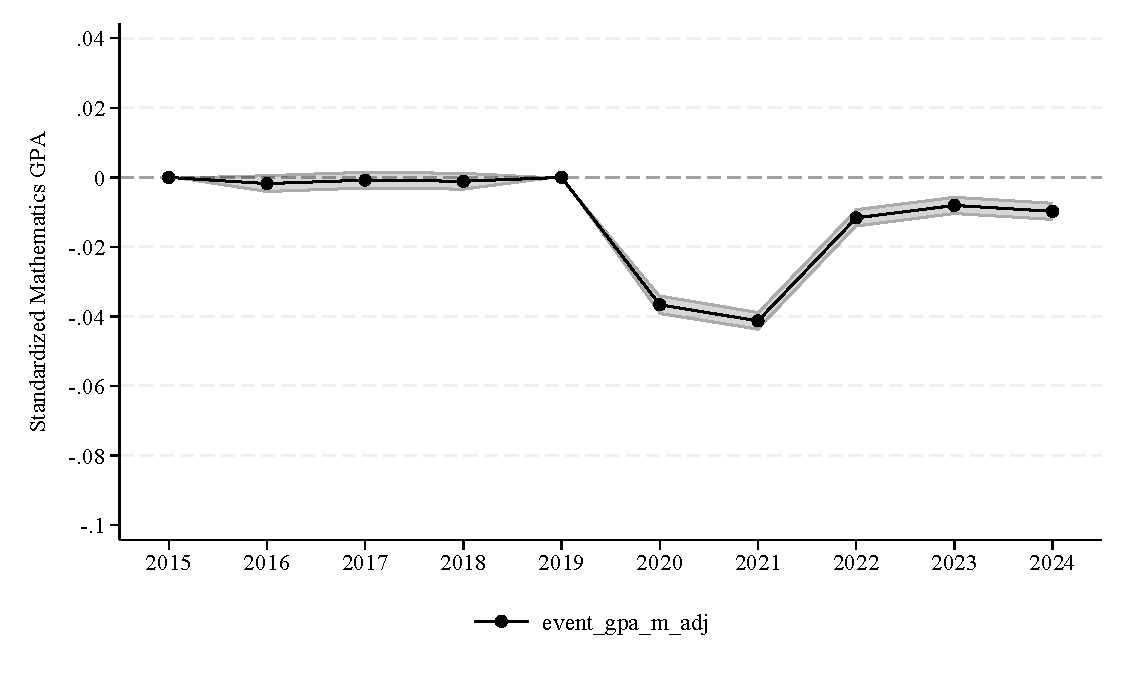
\includegraphics{./FIGURES/Event Study/covid_event_all_all_std_gpa_m_adj_Tsiblings_Sall_4.pdf}
      }
    }
\end{frame}

\begin{frame}
    \label{frame:eventstudy_bysibs}
    \frametitle{More siblings came with larger losses}
        {\resizebox{0.9\textwidth}{!}{
       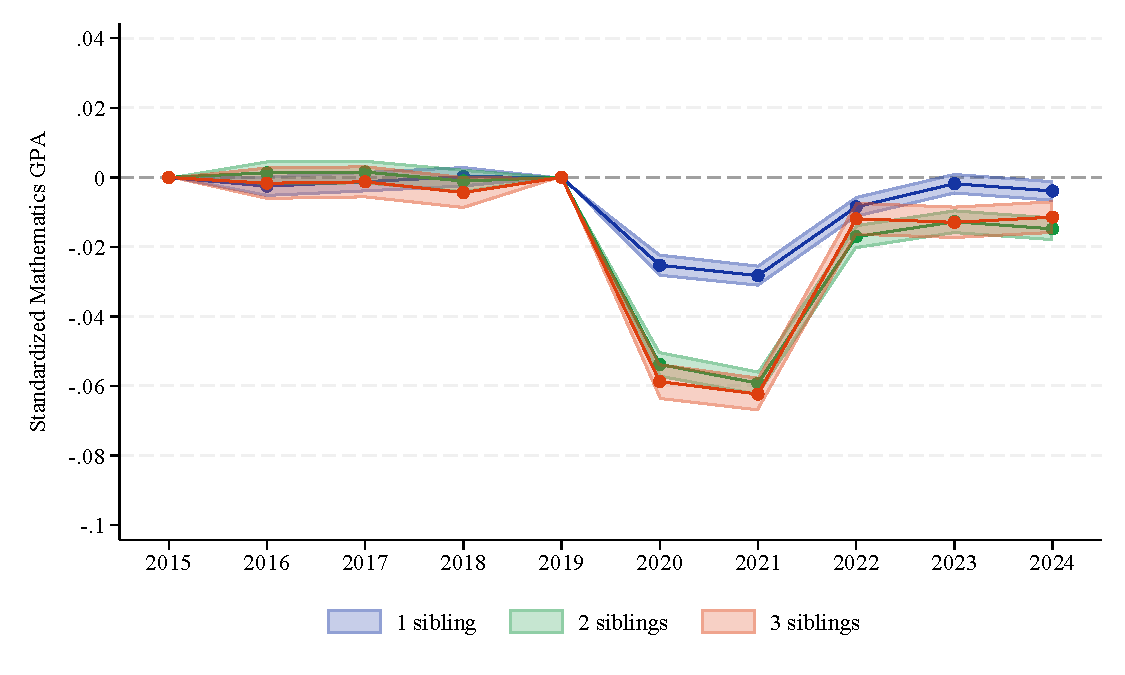
\includegraphics{./FIGURES/Event Study/covid_event_bysibs_all_all_std_gpa_m_adj_Tsiblings_Sall_4.pdf}
      }
    }
\end{frame}

\begin{frame}
    \label{frame:twfe_gpa_2_4_6_8}
    \frametitle{Differential learning losses are larger in earlier grades}
        {\resizebox{0.9\textwidth}{!}{
       %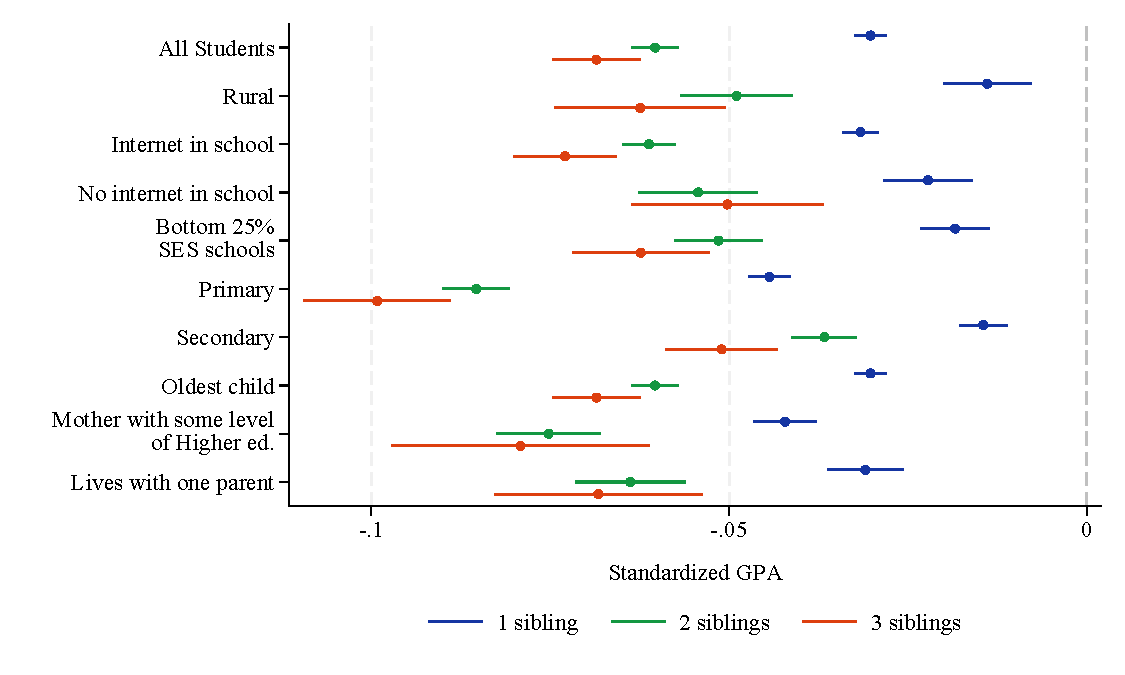
\includegraphics{./FIGURES/TWFE/covid_twfe_summ_bysibs_all_20-21_gpa_m_adj_Tsiblings_Soldest_4.pdf}
       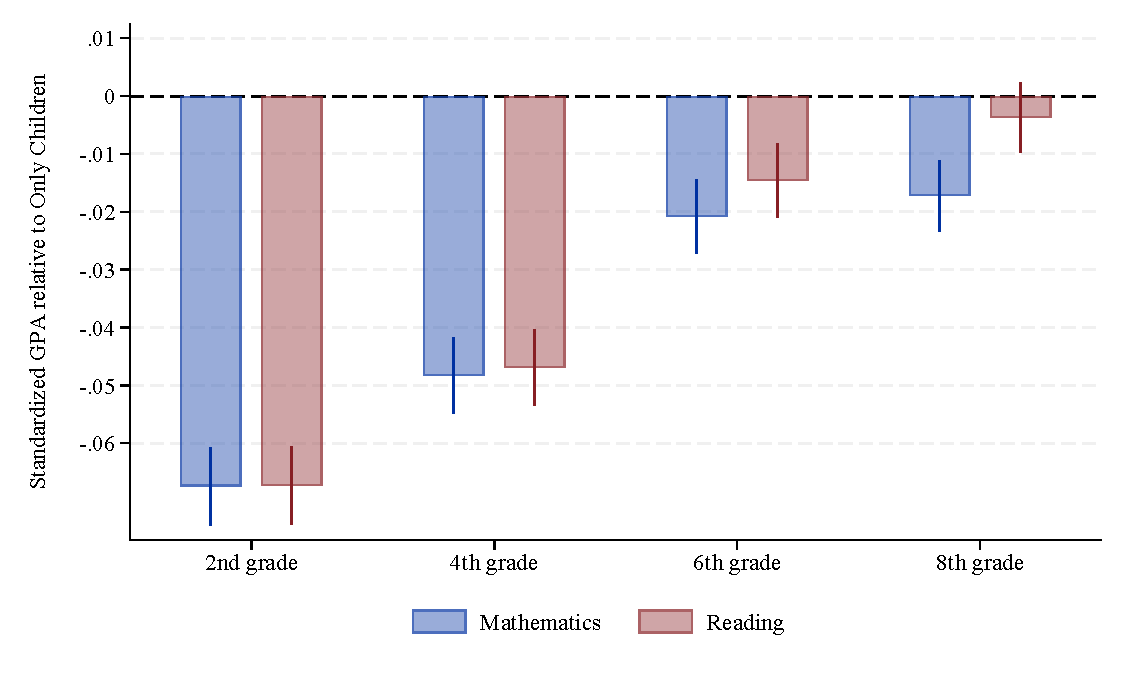
\includegraphics{./FIGURES/TWFE/twfe_gpa_2_4_6_8_20_21_Tsiblings_Soldest_4.pdf}
      }
    }
\end{frame}

\begin{frame}
    \label{frame:twfe_gpa_2_4_6_8}
    \frametitle{Losses in Standardized exams 2022-2024}
        {\resizebox{0.9\textwidth}{!}{
       %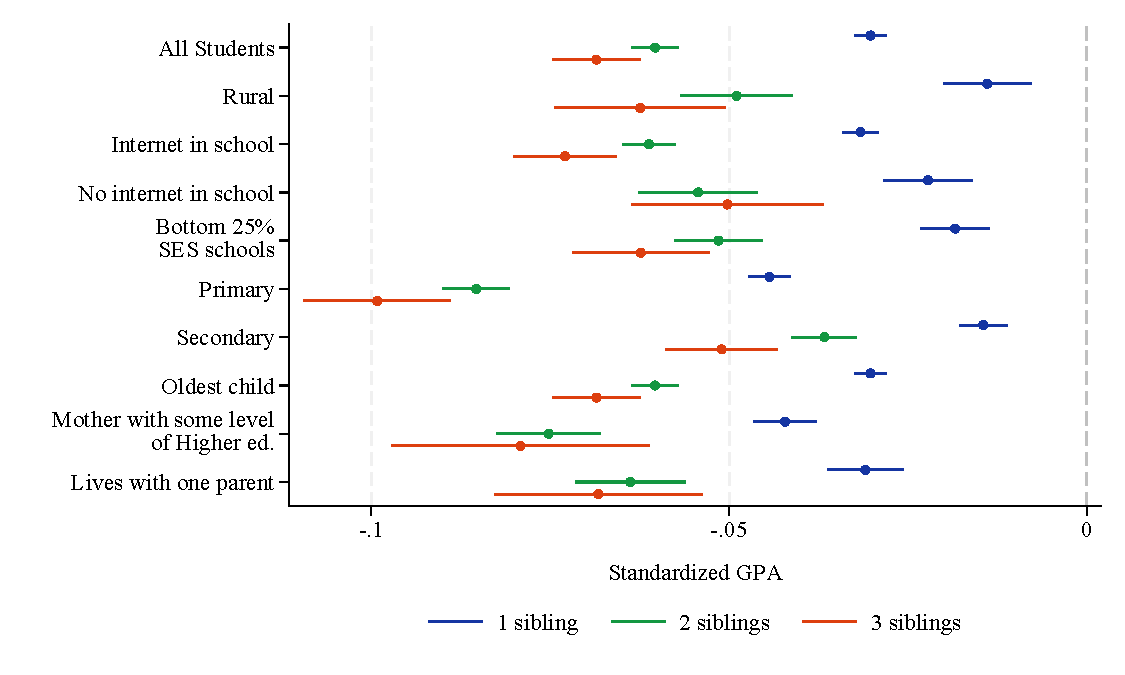
\includegraphics{./FIGURES/TWFE/covid_twfe_summ_bysibs_all_20-21_gpa_m_adj_Tsiblings_Soldest_4.pdf}
       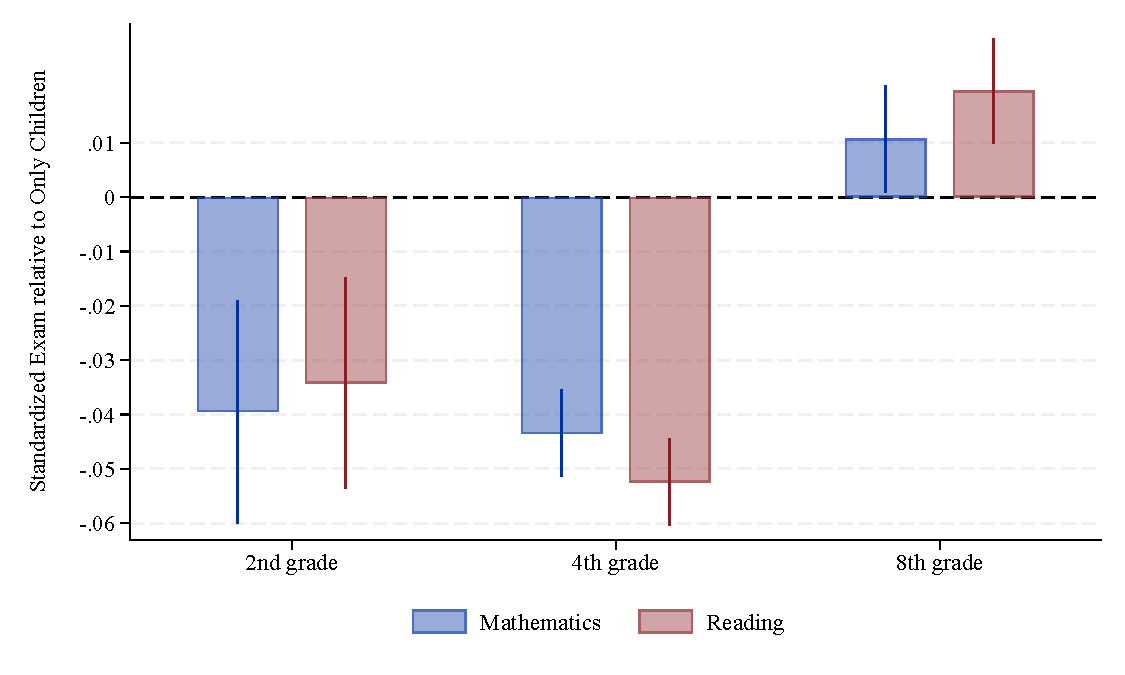
\includegraphics{./FIGURES/TWFE/twfe_ece_2_4_8_Tsiblings_Soldest_4.pdf}
      }
    }
\end{frame}


\begin{frame}
    \label{frame:birthorder}
    \frametitle{TWFE estimates for 2020-2021}
       \begin{itemize}
           \item Using the administrative data we can control for sex, mother's age, mother's age at first birth, mother's education and school, year and grade FE.
           %\item In some cases, I can use survey data for a more rich set of controls.
           \item For students in 6th, 7th and 9th grade, I can match baseline characteristics from 2nd, 4th and 8th grade.
           \item Similar results with standardized exams and socioeconomic index controls.


%    - 1. 2° (2015,2016) 					→ 6° (2019,2020)
%	- 2. 2° (2014,2016) + 4° (2016,2018) 	→ 6° (2018,2020)
%	- 3. 2° (2014,2016) + 4° (2016,2018) 	→ 7° (2019,2021)
%	- 4. 2° (2012,2013) + 8° (2018,2019) 	→ 9° (2019,2020)              
       \end{itemize}
\end{frame}


\begin{frame}
    \label{frame:twfe_gpa_controls}
    \frametitle{Results do not change when controlling for scores and socio-economic status}
        {\resizebox{0.9\textwidth}{!}{
       %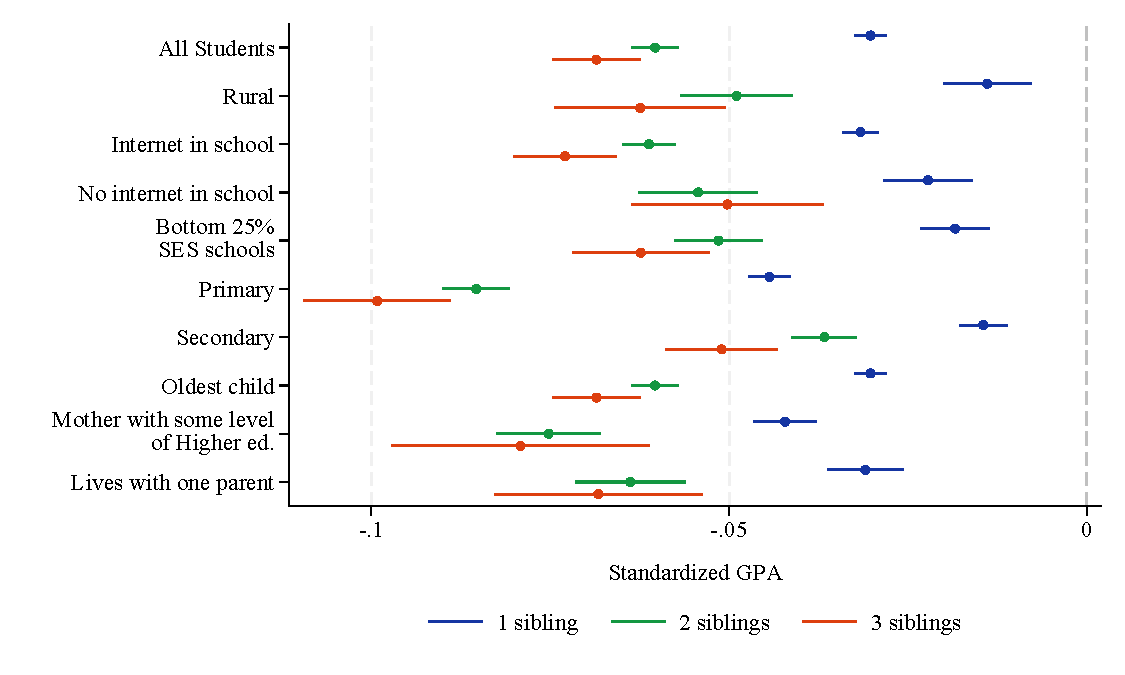
\includegraphics{./FIGURES/TWFE/covid_twfe_summ_bysibs_all_20-21_gpa_m_adj_Tsiblings_Soldest_4.pdf}
       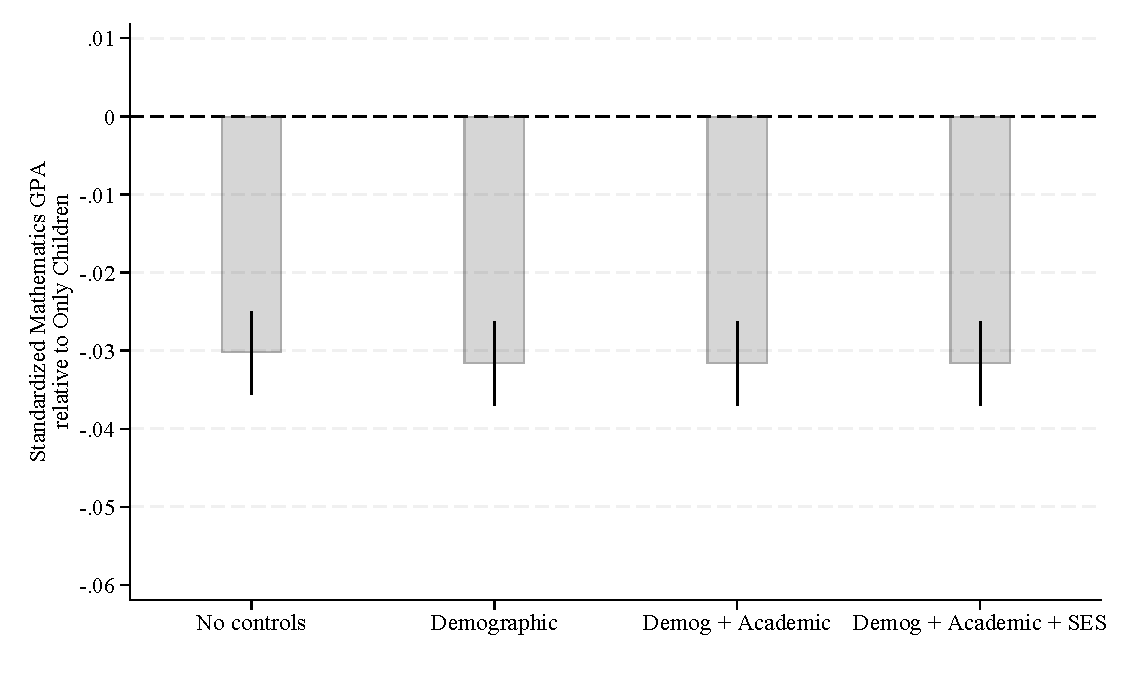
\includegraphics{./FIGURES/TWFE/twfe_std_gpa_m_adj_bycontrols_Tsiblings_Soldest_pairall_4.pdf}
      }
    }

      \begin{flushleft}
        \hyperlink{frame:twfe_gpa_controls_siblings}{\beamergotobutton{Results by siblings}}
        \hyperlink{frame:twfe_gpa_controls_1}{\beamergotobutton{6th-2nd grade}}
        \hyperlink{frame:twfe_gpa_controls_2}{\beamergotobutton{6th-4th grade}}
         \hyperlink{frame:twfe_gpa_controls_3}{\beamergotobutton{7th-4th grade}}
        \hyperlink{frame:twfe_gpa_controls_4}{\beamergotobutton{9th-8th grade}}  
    \end{flushleft}   
    
\end{frame}

\begin{frame}
    \label{frame:twfe_gpa_controls_siblings}
    \frametitle{Results do not change when controlling for scores and socio-economic status}
        {\resizebox{0.9\textwidth}{!}{
        %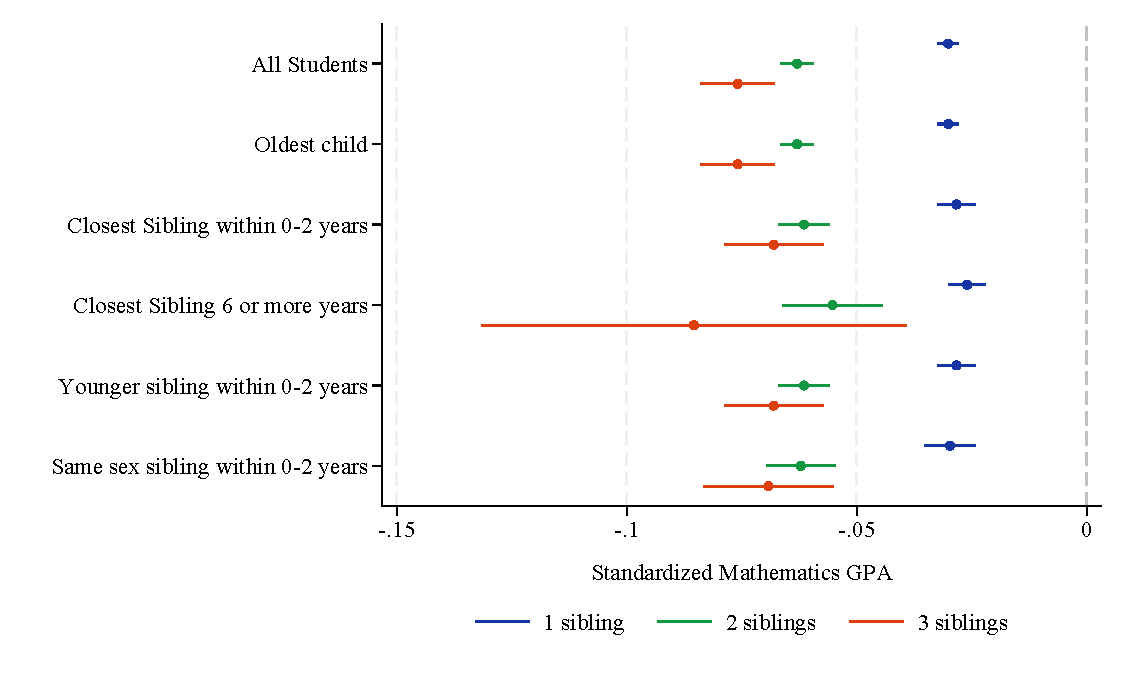
\includegraphics{./FIGURES/TWFE/covid_twfe_C_bysibs_elm_all_gpa_m_adj_Tsiblings_Soldest_4.pdf}
       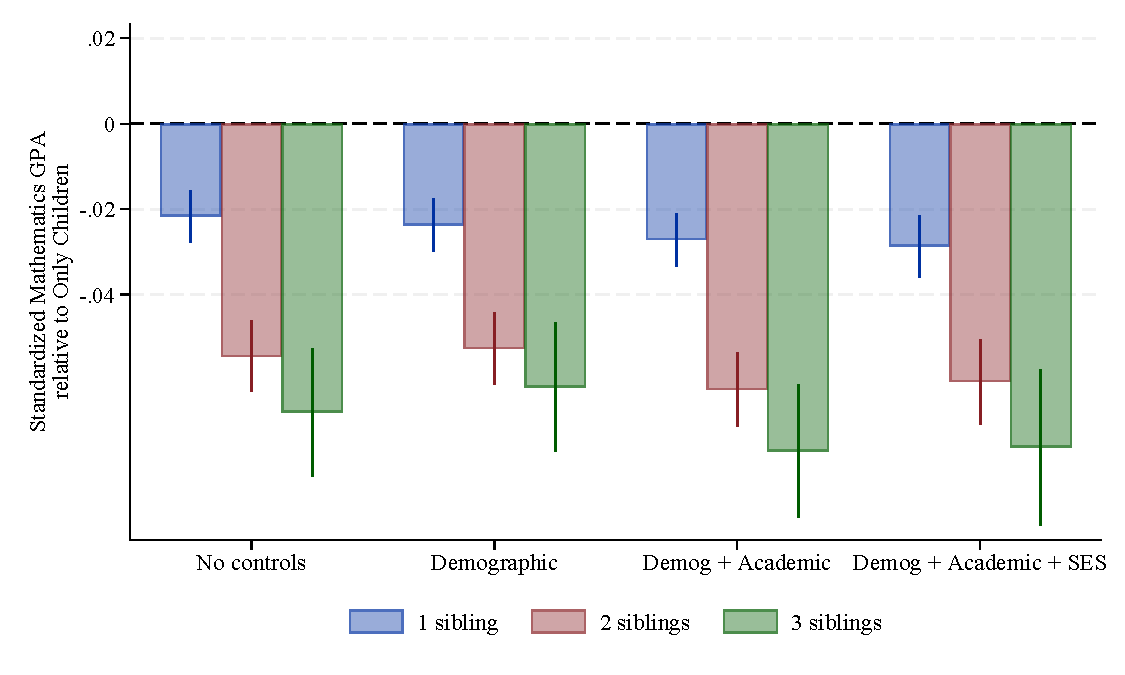
\includegraphics{./FIGURES/TWFE/twfe_std_gpa_m_adj_bycontrols_bysibs_Tsiblings_Soldest_pairall_4.pdf}
      }
    }

    \begin{flushleft}
        \hyperlink{frame:twfe_gpa_controls}{\beamergotobutton{Go Back $\carriagereturn$}}
    \end{flushleft}       

\end{frame}

\begin{frame}
    \label{frame:twfe_gpa_controls_1}
    \frametitle{6th graders with 2nd grade baseline}
        {\resizebox{0.9\textwidth}{!}{
       %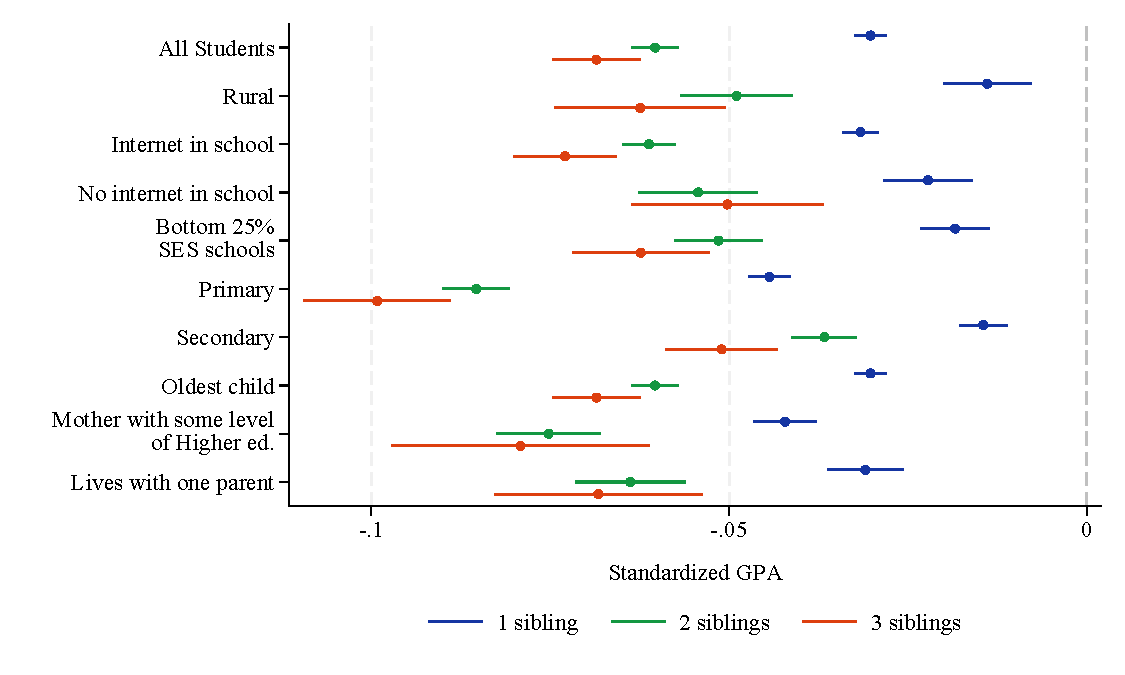
\includegraphics{./FIGURES/TWFE/covid_twfe_summ_bysibs_all_20-21_gpa_m_adj_Tsiblings_Soldest_4.pdf}
       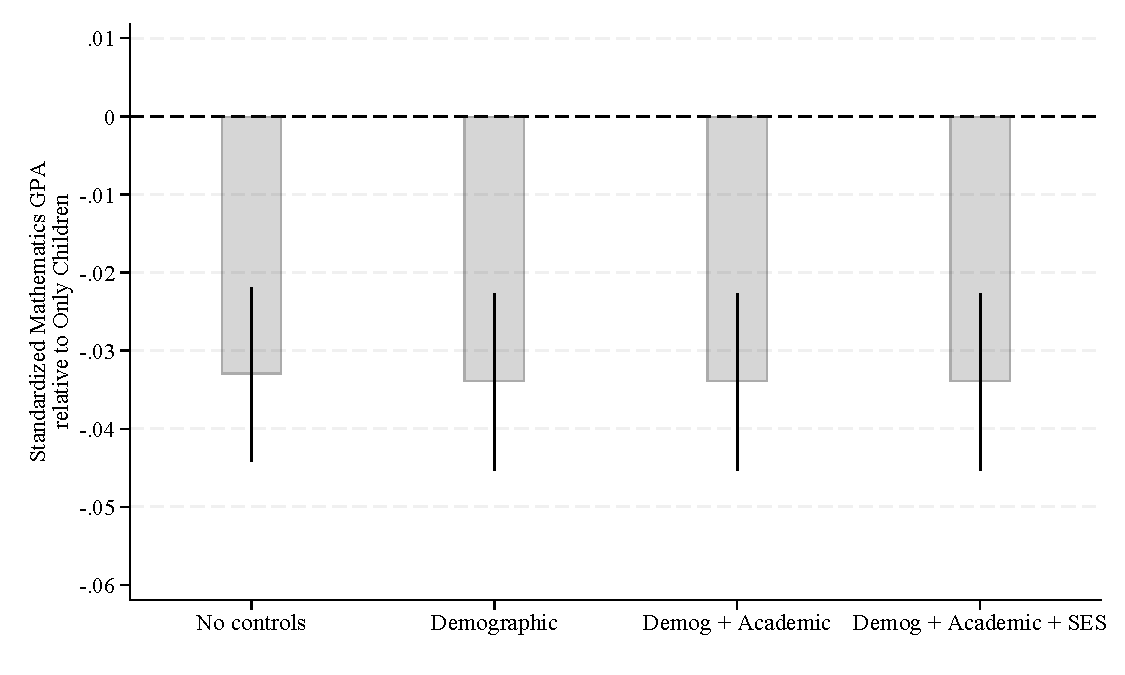
\includegraphics{./FIGURES/TWFE/twfe_std_gpa_m_adj_bycontrols_Tsiblings_Soldest_pair1_4.pdf}
      }
    }

    \begin{flushleft}
        \hyperlink{frame:twfe_gpa_controls}{\beamergotobutton{Go Back $\carriagereturn$}}
    \end{flushleft}       
\end{frame}

\begin{frame}
    \label{frame:twfe_gpa_controls_2}
    \frametitle{6th graders with 4th grade baseline}
        {\resizebox{0.9\textwidth}{!}{
       %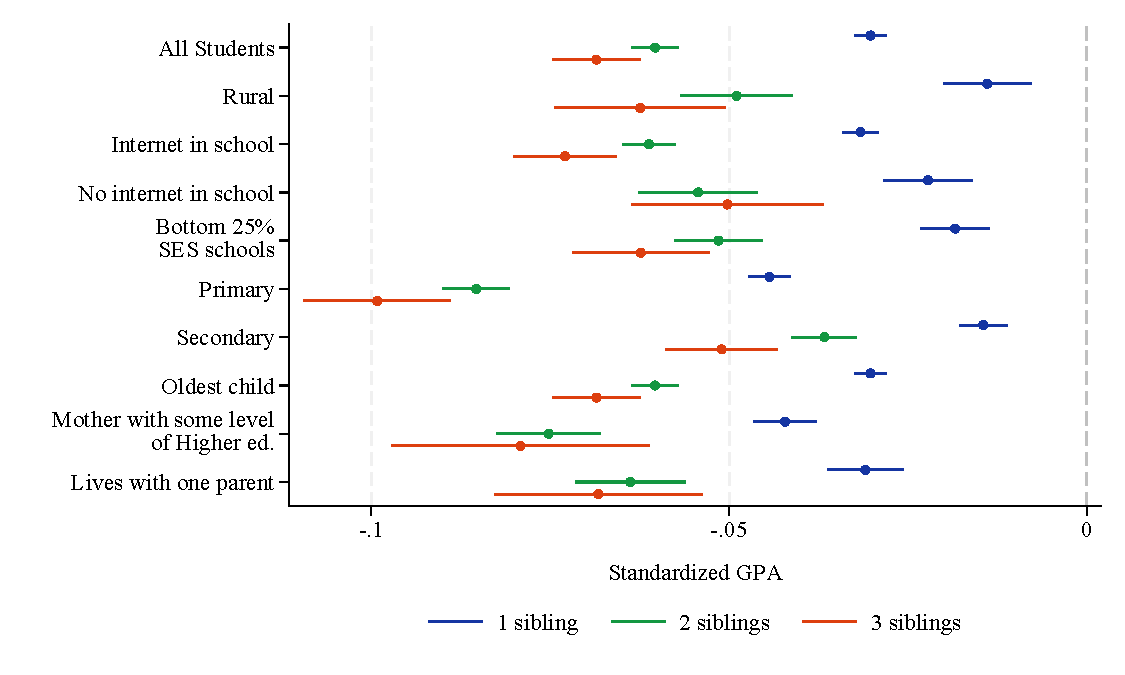
\includegraphics{./FIGURES/TWFE/covid_twfe_summ_bysibs_all_20-21_gpa_m_adj_Tsiblings_Soldest_4.pdf}
       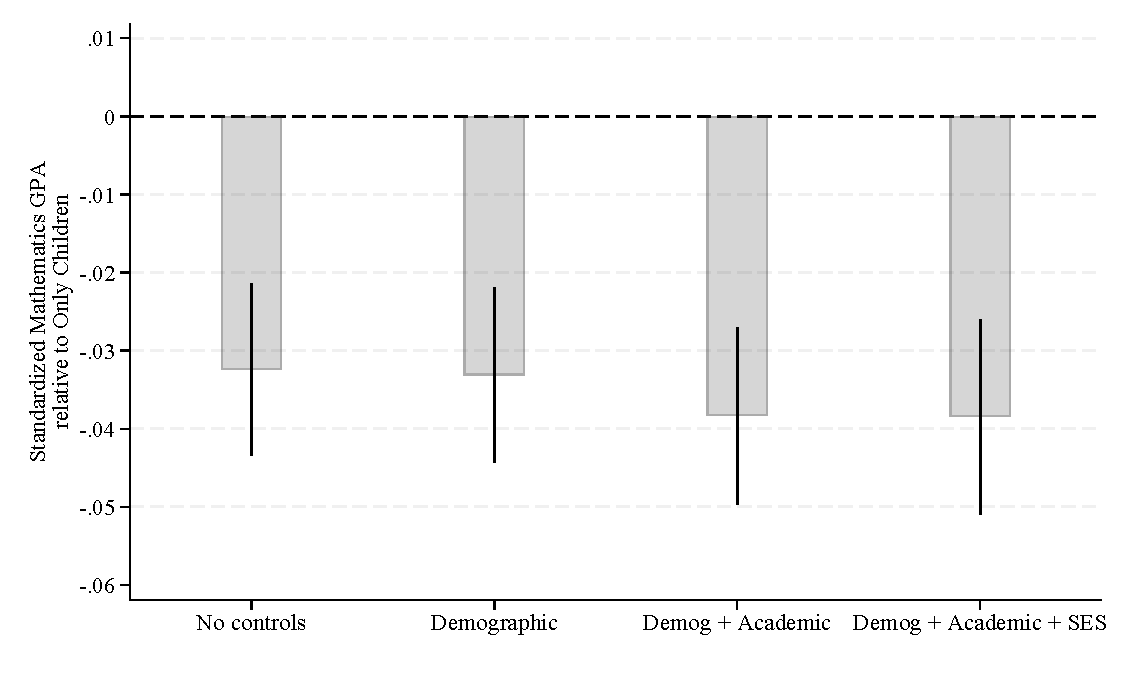
\includegraphics{./FIGURES/TWFE/twfe_std_gpa_m_adj_bycontrols_Tsiblings_Soldest_pair2_4.pdf}
      }
    }

    \begin{flushleft}
        \hyperlink{frame:twfe_gpa_controls}{\beamergotobutton{Go Back $\carriagereturn$}}
    \end{flushleft}       
\end{frame}

\begin{frame}
    \label{frame:twfe_gpa_controls_3}
    \frametitle{7th graders with 4th grade baseline}
        {\resizebox{0.9\textwidth}{!}{
       %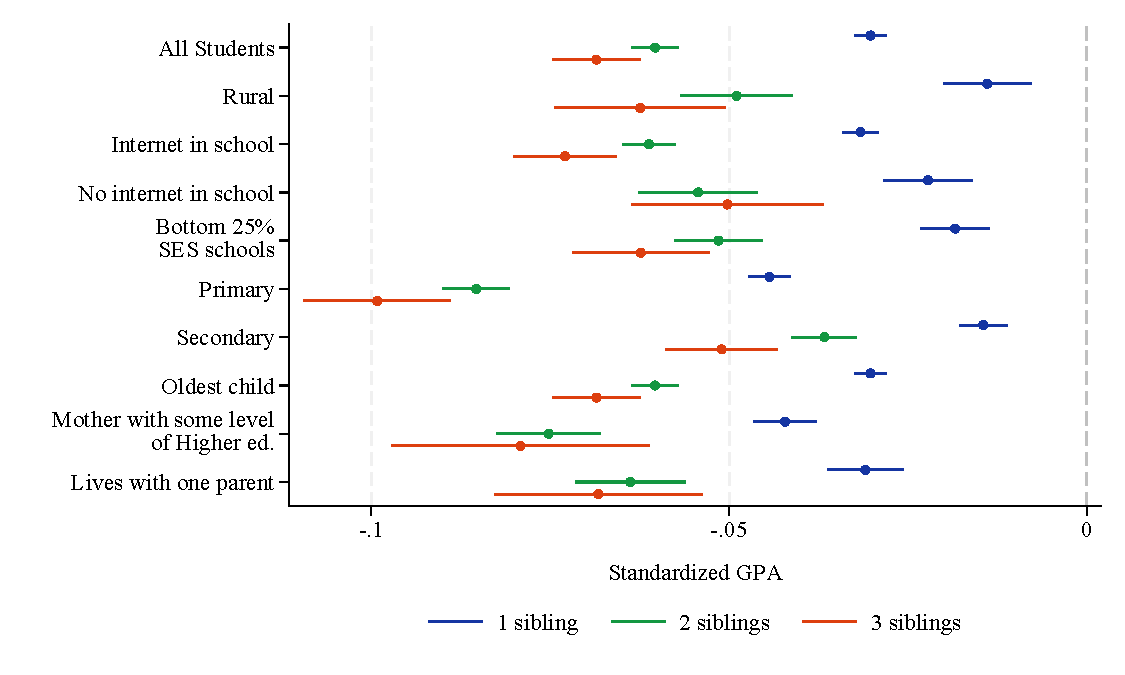
\includegraphics{./FIGURES/TWFE/covid_twfe_summ_bysibs_all_20-21_gpa_m_adj_Tsiblings_Soldest_4.pdf}
       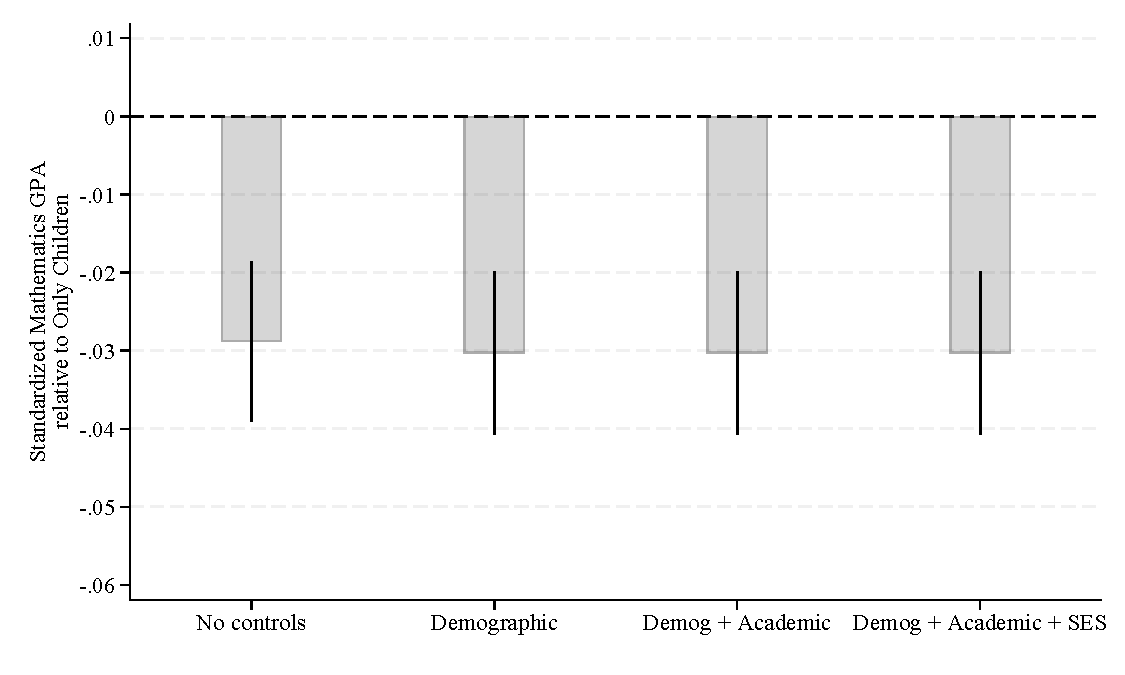
\includegraphics{./FIGURES/TWFE/twfe_std_gpa_m_adj_bycontrols_Tsiblings_Soldest_pair3_4.pdf}
      }
    }

    \begin{flushleft}
        \hyperlink{frame:twfe_gpa_controls}{\beamergotobutton{Go Back $\carriagereturn$}}
    \end{flushleft}       
\end{frame}

\begin{frame}
    \label{frame:twfe_gpa_controls_4}
    \frametitle{9th graders with 8th grade baseline}
        {\resizebox{0.9\textwidth}{!}{
       %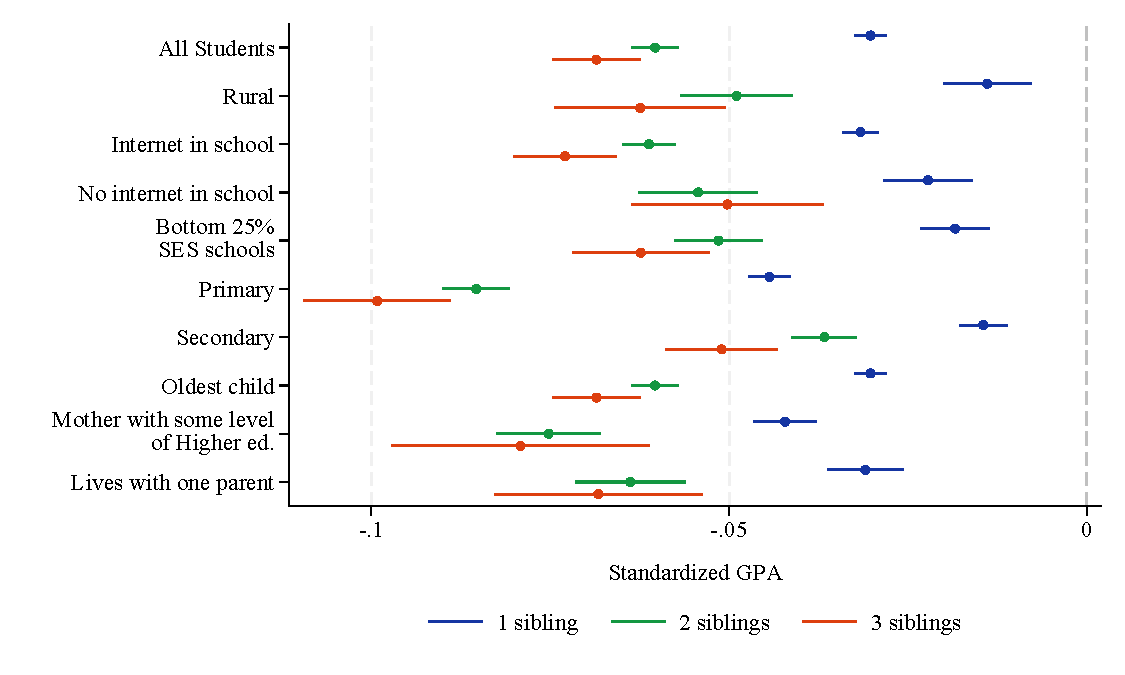
\includegraphics{./FIGURES/TWFE/covid_twfe_summ_bysibs_all_20-21_gpa_m_adj_Tsiblings_Soldest_4.pdf}
       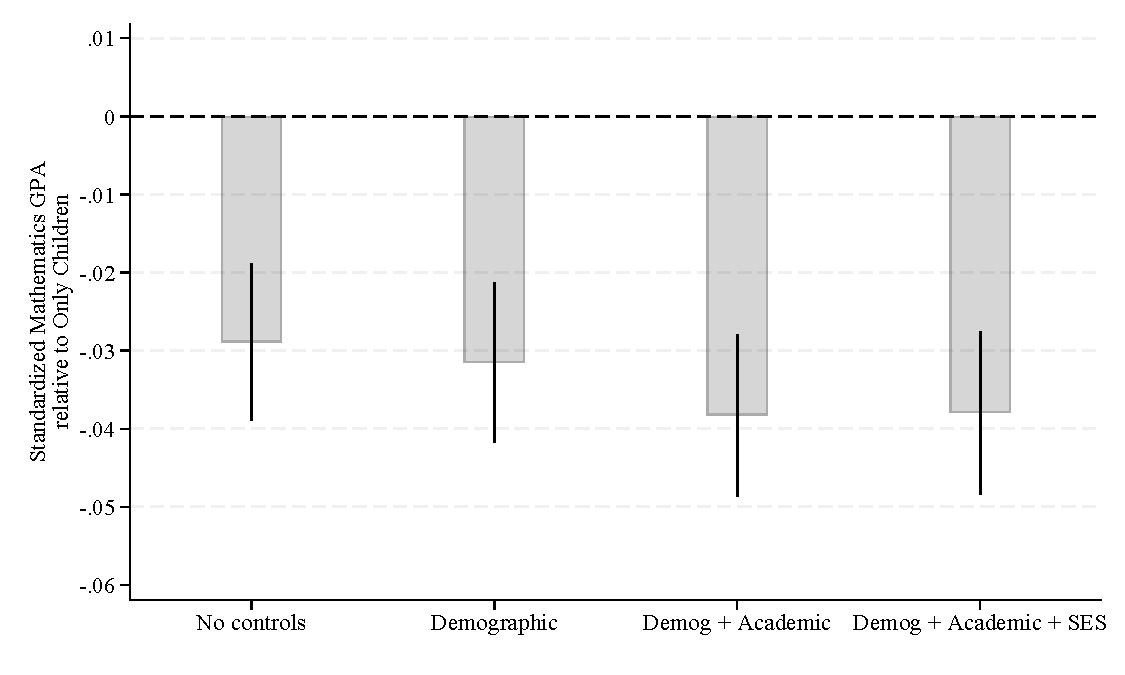
\includegraphics{./FIGURES/TWFE/twfe_std_gpa_m_adj_bycontrols_Tsiblings_Soldest_pair4_4.pdf}
      }
    }

    \begin{flushleft}
        \hyperlink{frame:twfe_gpa_controls}{\beamergotobutton{Go Back $\carriagereturn$}}
    \end{flushleft}       
\end{frame}


% ========================================
% MECHANISMS
% ========================================
\begin{frame}
    \label{frame:mechanisms}
    \frametitle{What's behind this?}
\begin{itemize}
    \item Having a sibling is related with larger learning losses.
    \item Students interact less with teachers and peers and more with parents and siblings.
    \item Potential Mechanisms:   
    \begin{itemize}
        \item Birth Order
        \item Scarce material resources
        \item Sibling disruption
        \item Parental dilution
        \item Income Shocks
    \end{itemize} 
\end{itemize}
\end{frame}

\begin{frame}
    \label{frame:birthorder}
    \frametitle{Birth Order}
       \begin{itemize}
           \item Effects of school closures may be different for 1st, 2nd, 3rd... children.
           \item This is different from family size effects.
           \item In order to separate both, we only consider first-born children.
       \end{itemize}
\end{frame}

\begin{frame}
    \label{frame:birthorder_intro}
    \frametitle{Birth Order}
        {\resizebox{0.9\textwidth}{!}{ 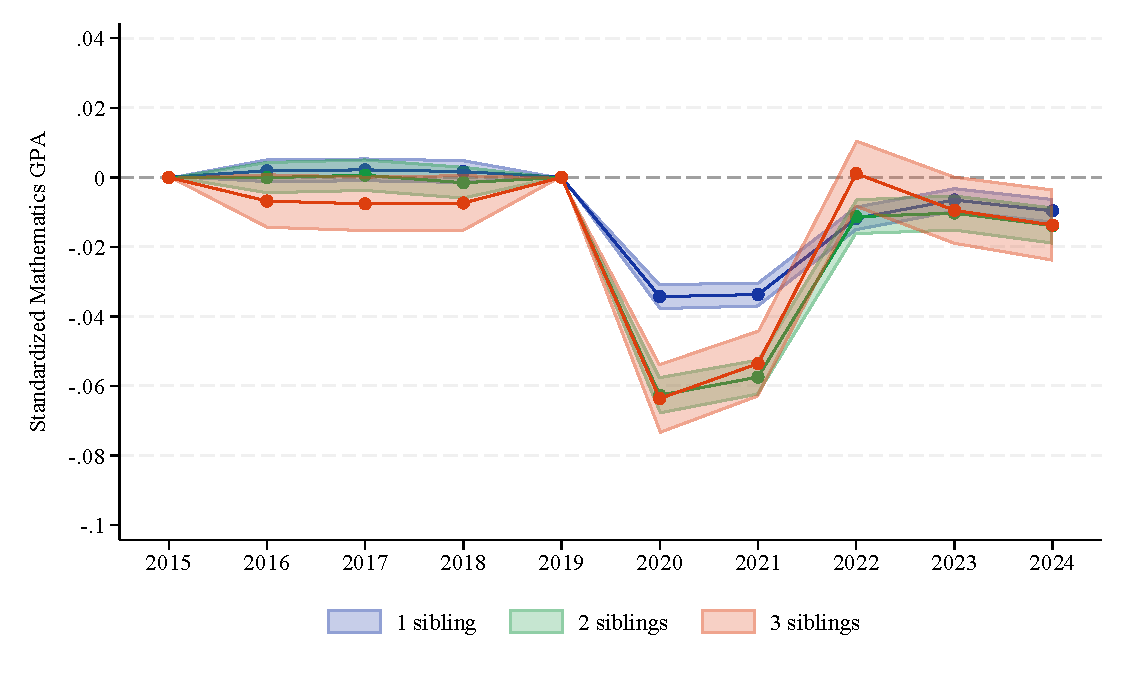
\includegraphics{./FIGURES/Event Study/covid_event_bysibs_all_all_std_gpa_m_adj_Tsiblings_Soldest_4.pdf}
      }
    }  

    \begin{flushleft}
        \hyperlink{frame:mechanisms}{\beamergotobutton{Mechanisms}}
    \end{flushleft}
\end{frame}


\begin{frame}
    \label{frame:resources_intro}
    \frametitle{Material Resources}
       \begin{itemize}
           \item Siblings may be competing for a computer to study
           \item But households without neither computer nor internet show similar patterns 
       \end{itemize}
\end{frame}


\begin{frame}
    \label{frame:pcinternet}
    \frametitle{PC and internet}
        {\resizebox{0.9\textwidth}{!}{
        %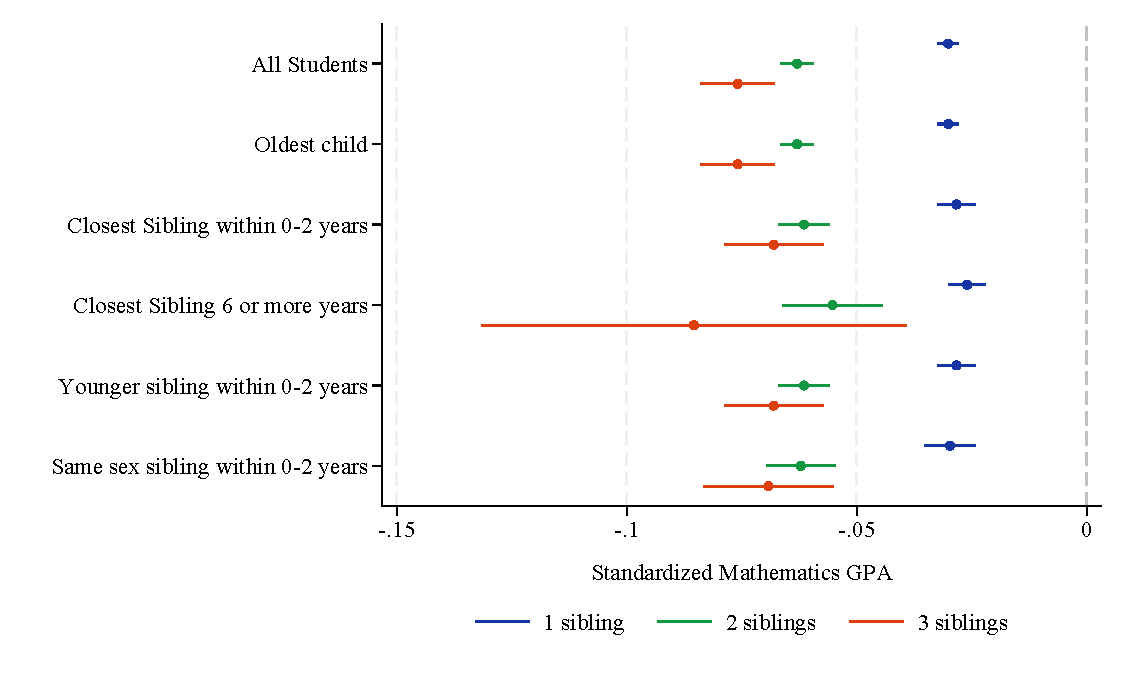
\includegraphics{./FIGURES/TWFE/covid_twfe_C_bysibs_elm_all_gpa_m_adj_Tsiblings_Soldest_4.pdf}
        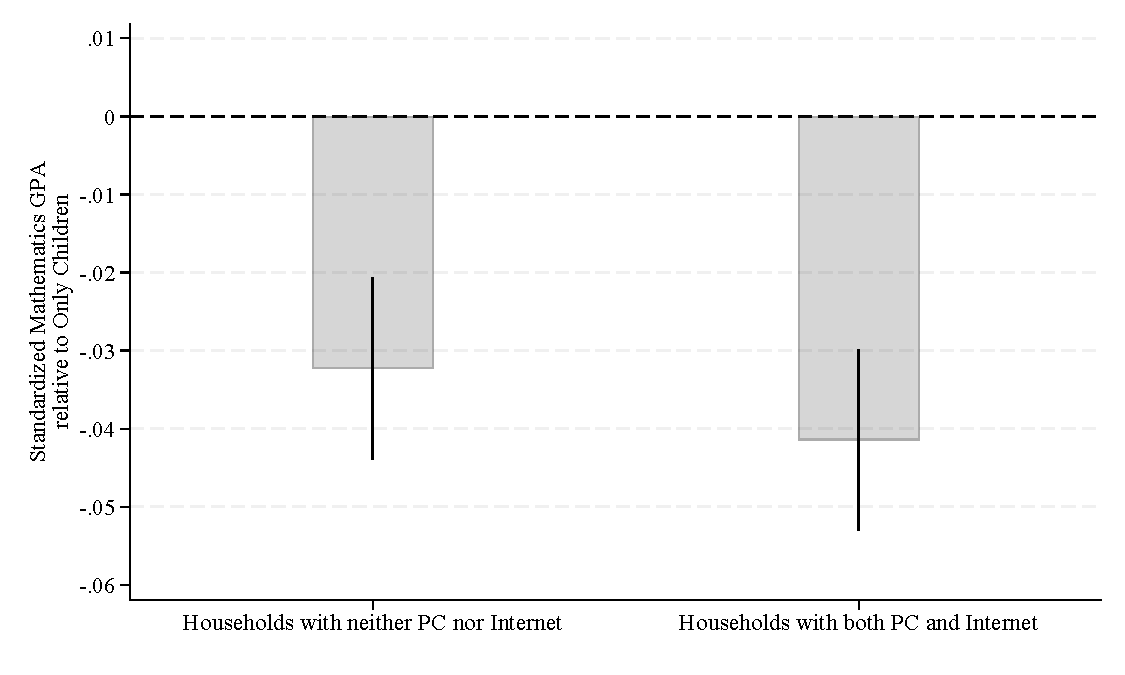
\includegraphics{./FIGURES/TWFE/twfe_std_gpa_m_adj_bypc_int_Tsiblings_Soldest_pairall_4.pdf}
      }
    }

    \begin{flushleft}
        \hyperlink{frame:pcinternet_siblings}{\beamergotobutton{Results by siblings}}
    \end{flushleft}    

\end{frame}

\begin{frame}
    \label{frame:pcinternet_siblings}
    \frametitle{PC and internet}
        {\resizebox{0.9\textwidth}{!}{
        %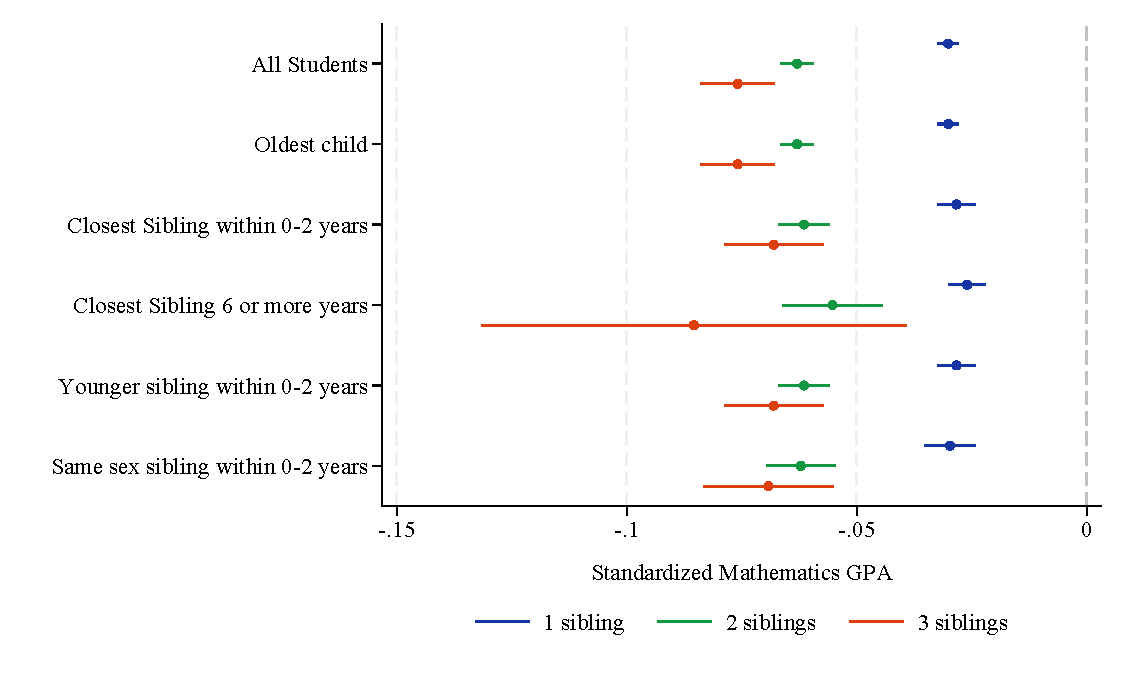
\includegraphics{./FIGURES/TWFE/covid_twfe_C_bysibs_elm_all_gpa_m_adj_Tsiblings_Soldest_4.pdf}
        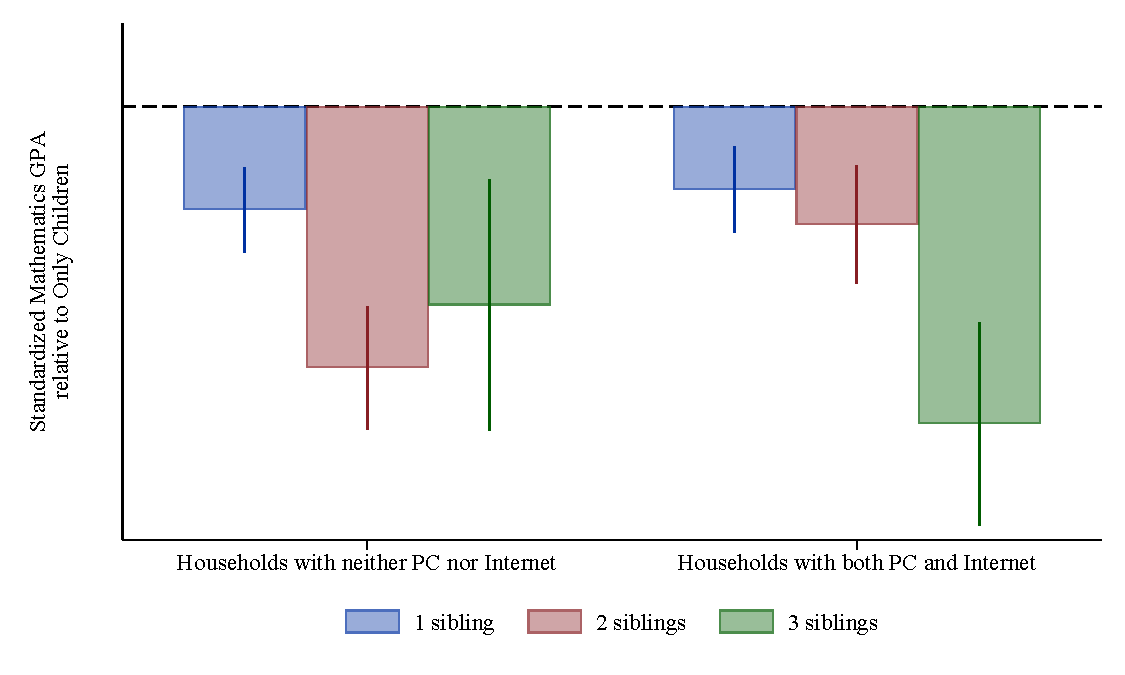
\includegraphics{./FIGURES/TWFE/twfe_std_gpa_m_adj_bypc_int_bysibs_Tsiblings_Soldest_pairall_4.pdf}
      }
    }

    \begin{flushleft}
        \hyperlink{frame:pcinternet}{\beamergotobutton{Go Back $\carriagereturn$}}
    \end{flushleft}       

\end{frame}



\begin{frame}
    \label{frame:siblingdisruption}
    \frametitle{Sibling disruption}
        {\resizebox{0.9\textwidth}{!}{
        %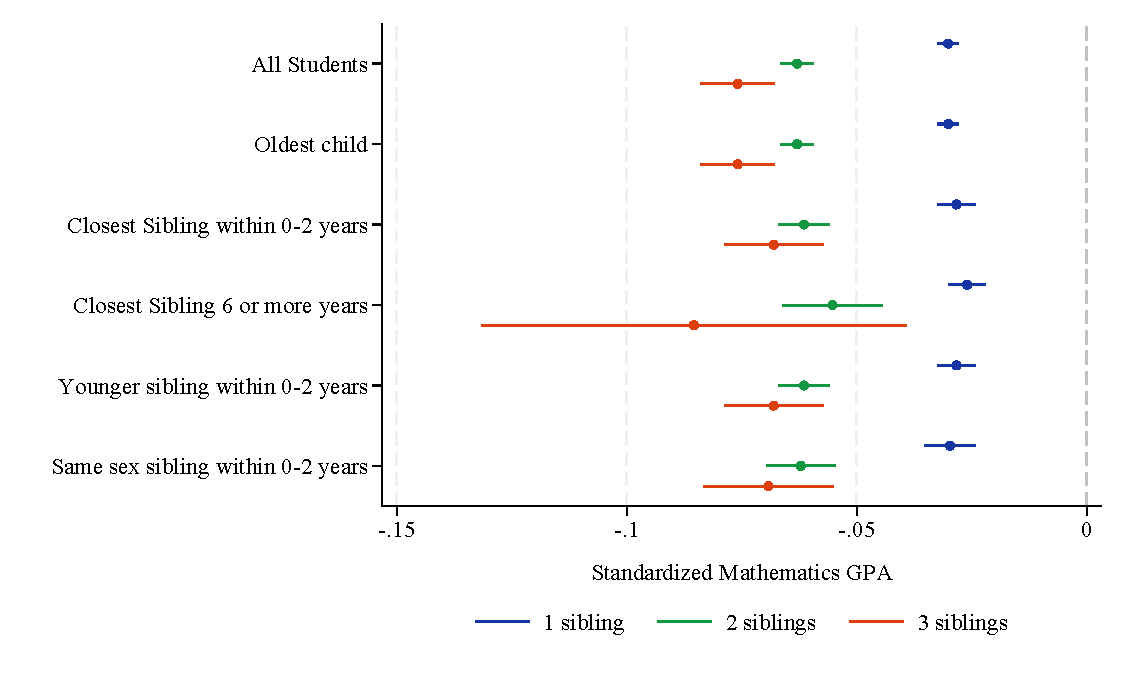
\includegraphics{./FIGURES/TWFE/covid_twfe_C_bysibs_elm_all_gpa_m_adj_Tsiblings_Soldest_4.pdf}
        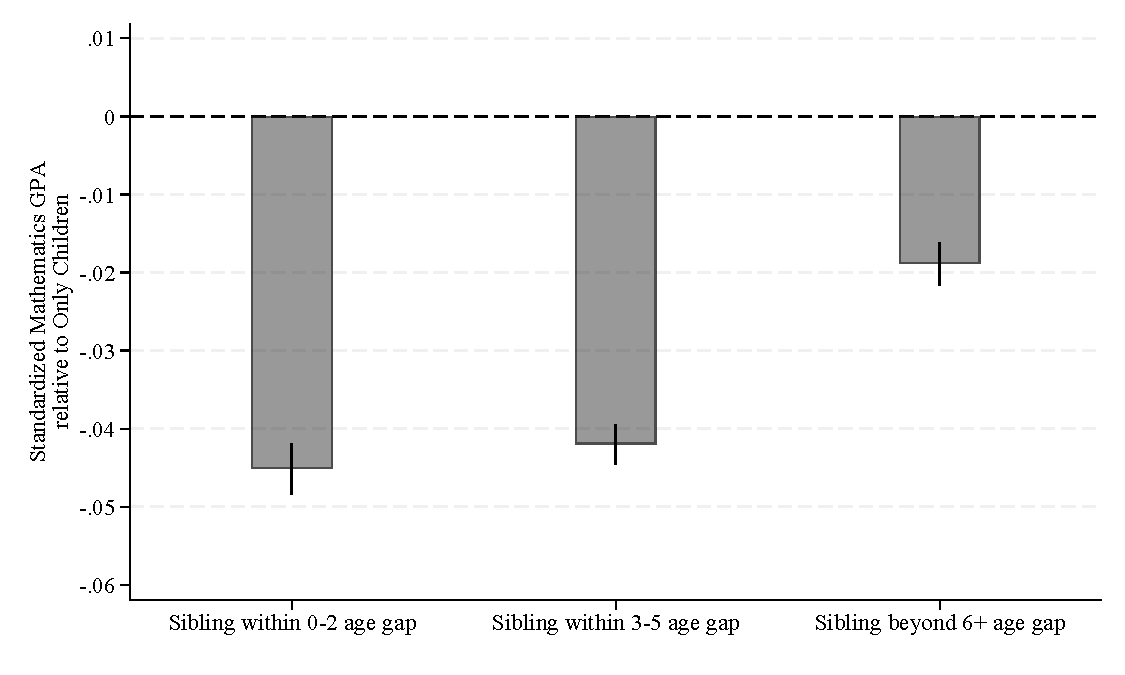
\includegraphics{./FIGURES/TWFE/twfe_gpa_age_gap_20_21_Tsiblings_Soldest_4.pdf}
      }
    }

    \begin{flushleft}
        \hyperlink{frame:siblingdisruption_siblings}{\beamergotobutton{Results by siblings}}
    \end{flushleft}    

\end{frame}

\begin{frame}
    \label{frame:siblingdisruption_siblings}
    \frametitle{Sibling disruption}
        {\resizebox{0.9\textwidth}{!}{
        %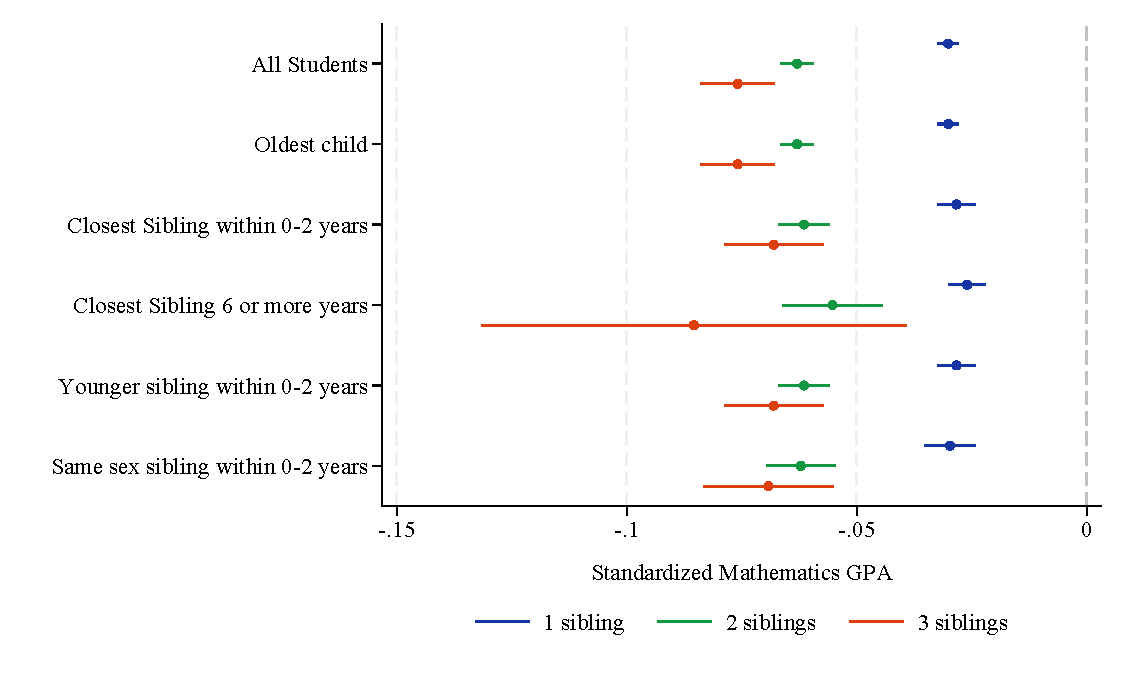
\includegraphics{./FIGURES/TWFE/covid_twfe_C_bysibs_elm_all_gpa_m_adj_Tsiblings_Soldest_4.pdf}
        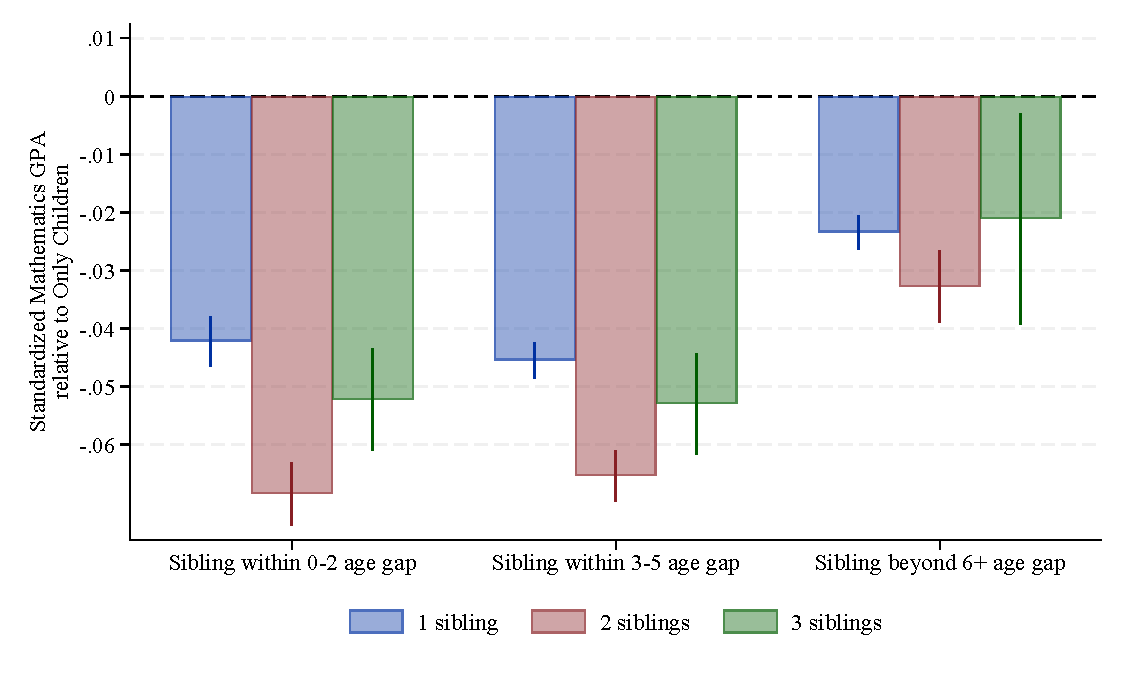
\includegraphics{./FIGURES/TWFE/twfe_gpa_age_gap_bysibs_20_21_Tsiblings_Soldest_4.pdf}
      }
    }

    \begin{flushleft}
        \hyperlink{frame:siblingdisruption}{\beamergotobutton{Go Back $\carriagereturn$}}
    \end{flushleft}        

\end{frame}





\begin{frame}
    \label{frame:parentaldilution_intro}
    \frametitle{Parental Resources}
       \begin{itemize}
           \item Parent's loose childcare and school support.
           \item Without pre-k or children in school, they need to take up on childcare.
           \item Additionally, they may need to provide help with schoolwork.
           \item ``Parents who before the pandemic invested time and resources in their children use official education resources the most... because of the employment  disruptions of the pandemic, they \textbf{[low SES]} spent  even less time during the lockdowns.'' \cite{naslund-hadley_education_2021}
       \end{itemize}
\end{frame}

\begin{frame}
    \label{frame:parental_investments_vs_ses}
    \frametitle{Parental time Investment increases with SES}
        {\resizebox{0.9\textwidth}{!}{
        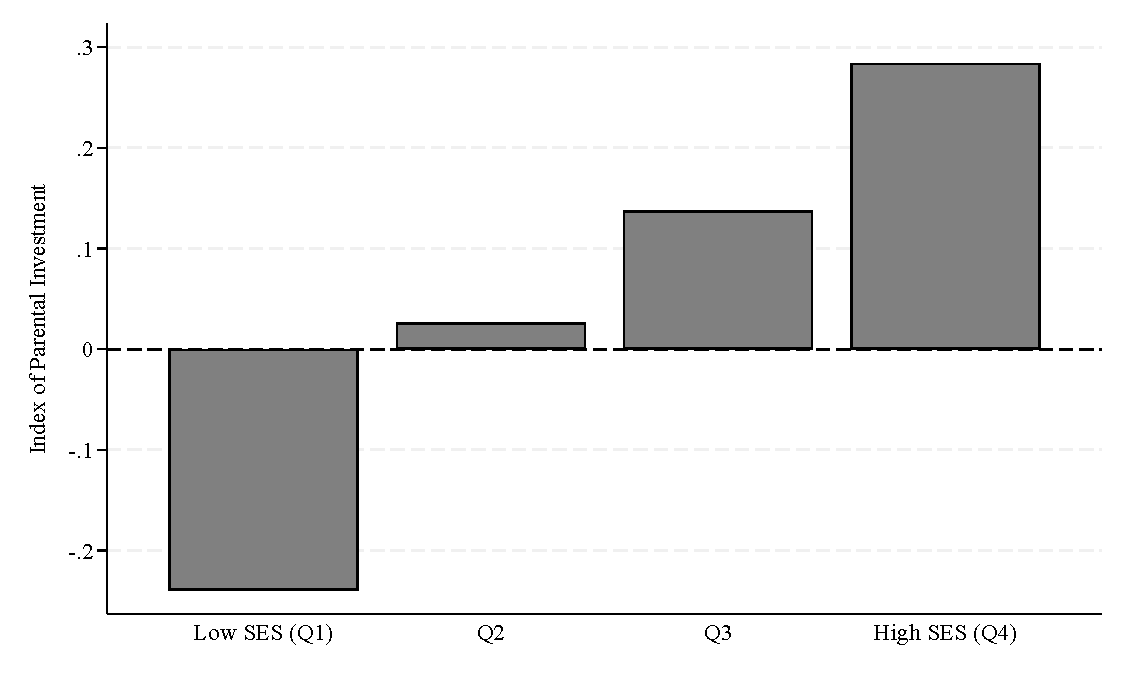
\includegraphics{./FIGURES/Descriptive/parental_investment_ses.pdf}
      }
    }

\end{frame}


\begin{frame}
    \label{frame:byses}
    \frametitle{Socio-Economic Status}
        {\resizebox{0.9\textwidth}{!}{
        %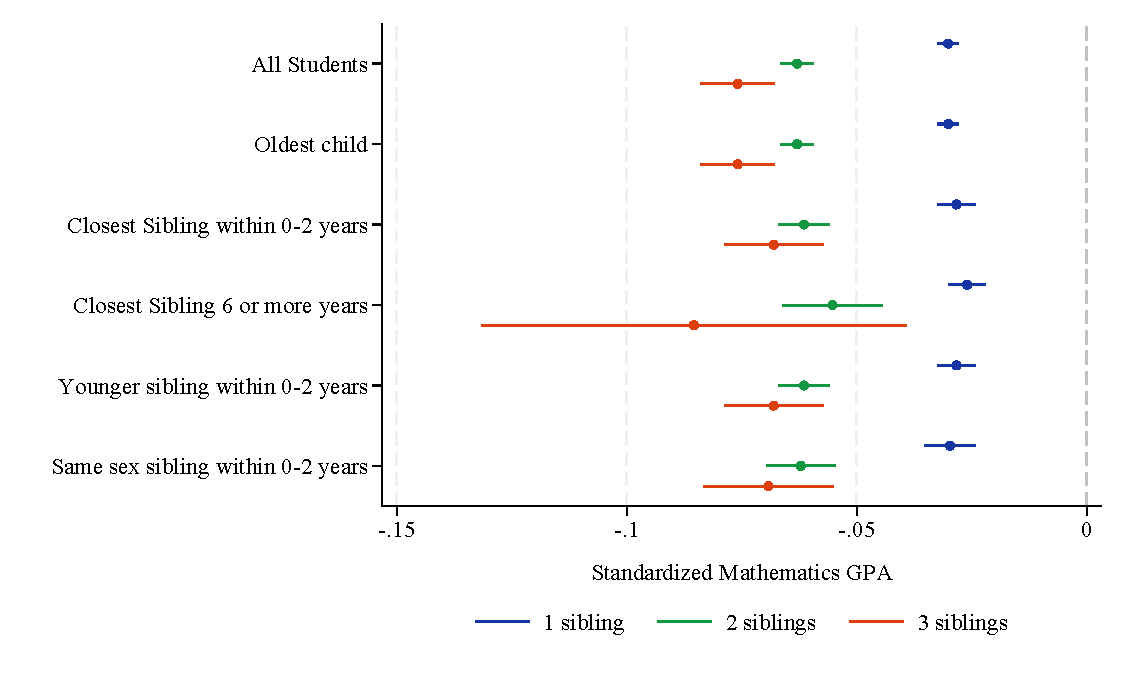
\includegraphics{./FIGURES/TWFE/covid_twfe_C_bysibs_elm_all_gpa_m_adj_Tsiblings_Soldest_4.pdf}
        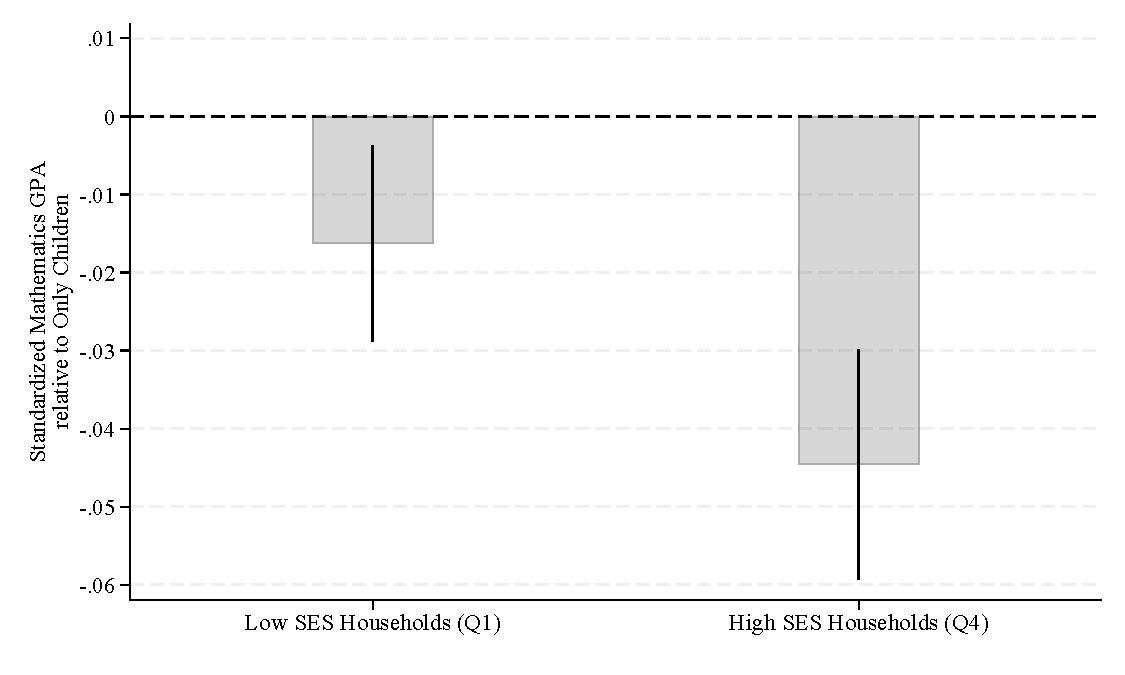
\includegraphics{./FIGURES/TWFE/twfe_std_gpa_m_adj_byses_Tsiblings_Soldest_pairall_4.pdf}
      }
    }

    \begin{flushleft}
        \hyperlink{frame:byses_siblings}{\beamergotobutton{Results by siblings}}
    \end{flushleft}    

\end{frame}

\begin{frame}
    \label{frame:byses_siblings}
    \frametitle{Socio-Economic Status}
        {\resizebox{0.9\textwidth}{!}{
        %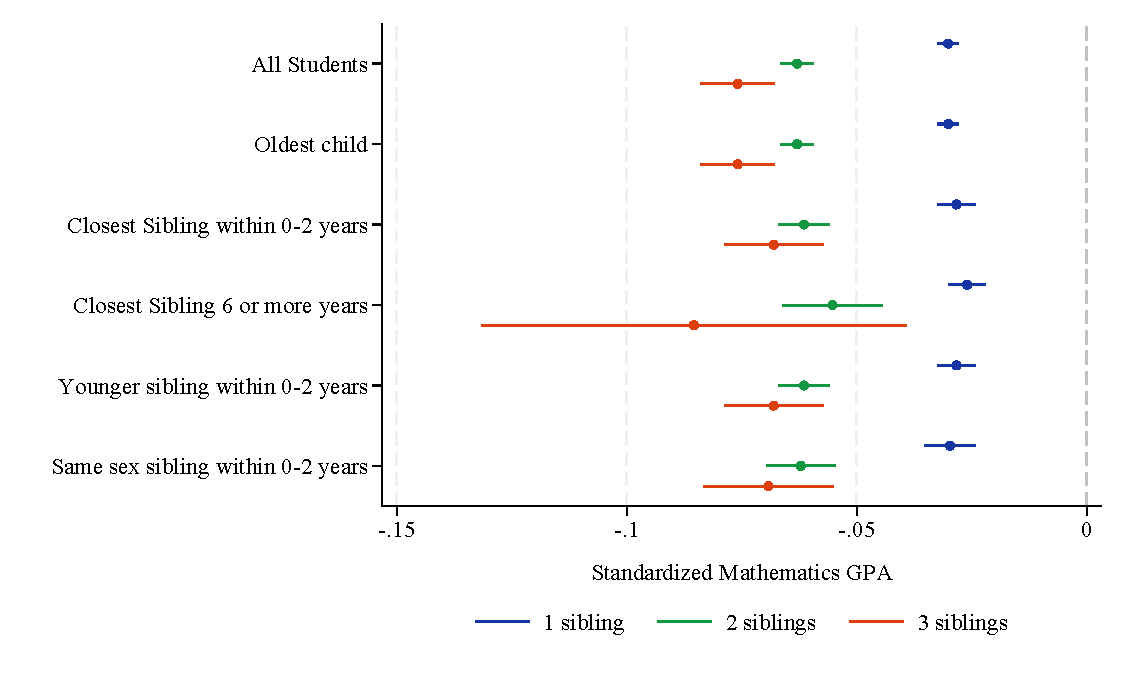
\includegraphics{./FIGURES/TWFE/covid_twfe_C_bysibs_elm_all_gpa_m_adj_Tsiblings_Soldest_4.pdf}
        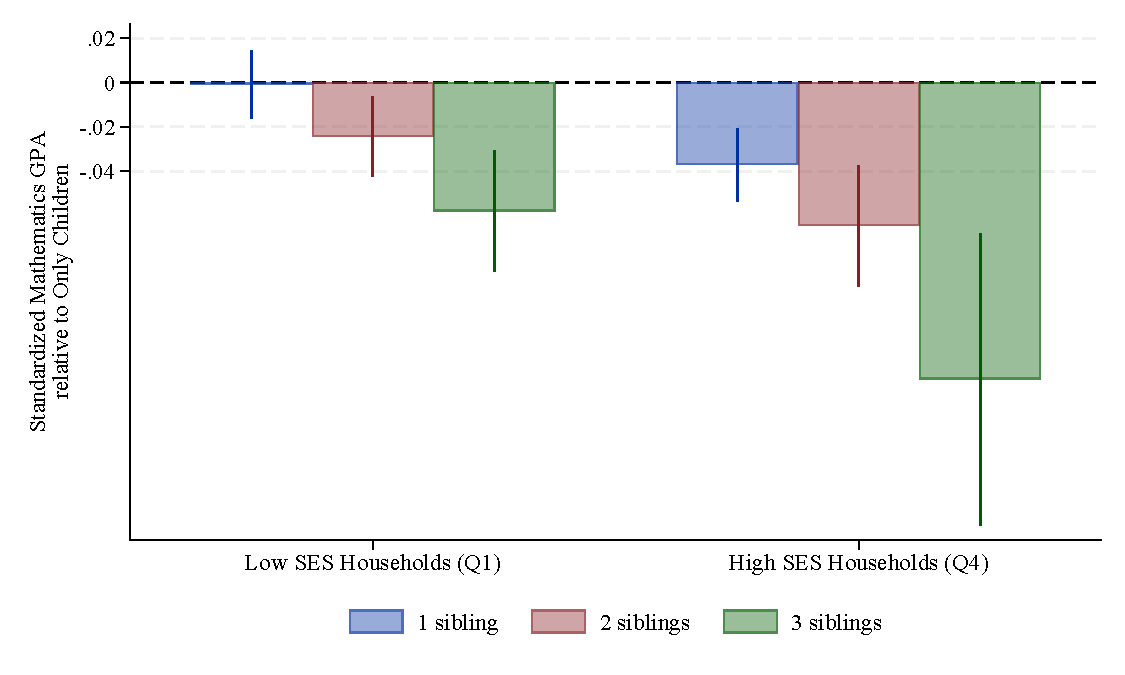
\includegraphics{./FIGURES/TWFE/twfe_std_gpa_m_adj_byses_bysibs_Tsiblings_Soldest_pairall_4.pdf}
      }
    }

    \begin{flushleft}
        \hyperlink{frame:byses}{\beamergotobutton{Go Back $\carriagereturn$}}
    \end{flushleft}        

\end{frame}



\begin{frame}
    \label{frame:mothereduc}
    \frametitle{Mother's Education}
        {\resizebox{0.9\textwidth}{!}{
        %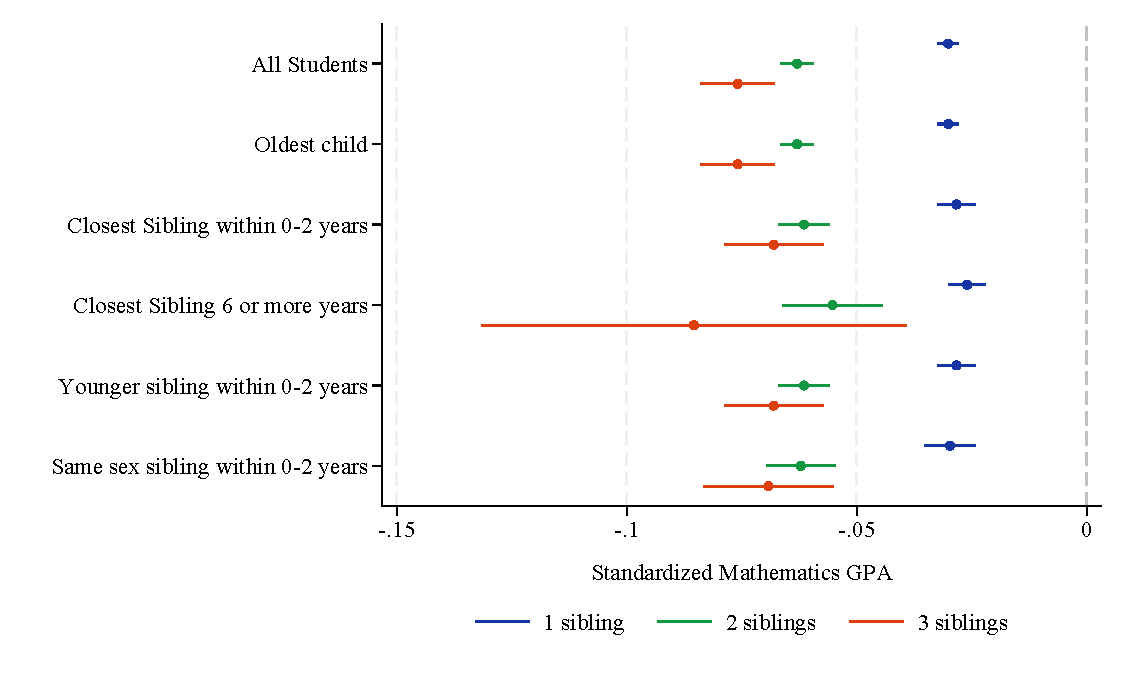
\includegraphics{./FIGURES/TWFE/covid_twfe_C_bysibs_elm_all_gpa_m_adj_Tsiblings_Soldest_4.pdf}
        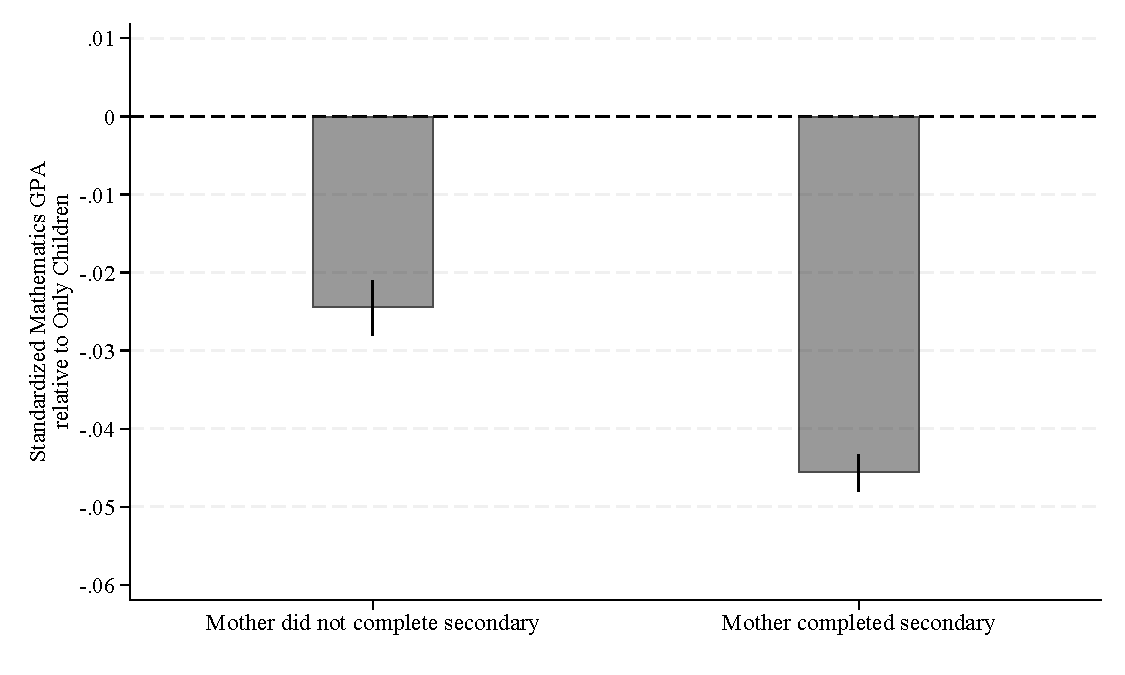
\includegraphics{./FIGURES/TWFE/twfe_gpa_mom_sec_complete_20_21_Tsiblings_Soldest_4.pdf}
      }
    }

    \begin{flushleft}
        \hyperlink{frame:mothereduc_siblings}{\beamergotobutton{Results by siblings}}
    \end{flushleft}    

\end{frame}

\begin{frame}
    \label{frame:mothereduc_siblings}
    \frametitle{Mother's Education}
        {\resizebox{0.9\textwidth}{!}{
        %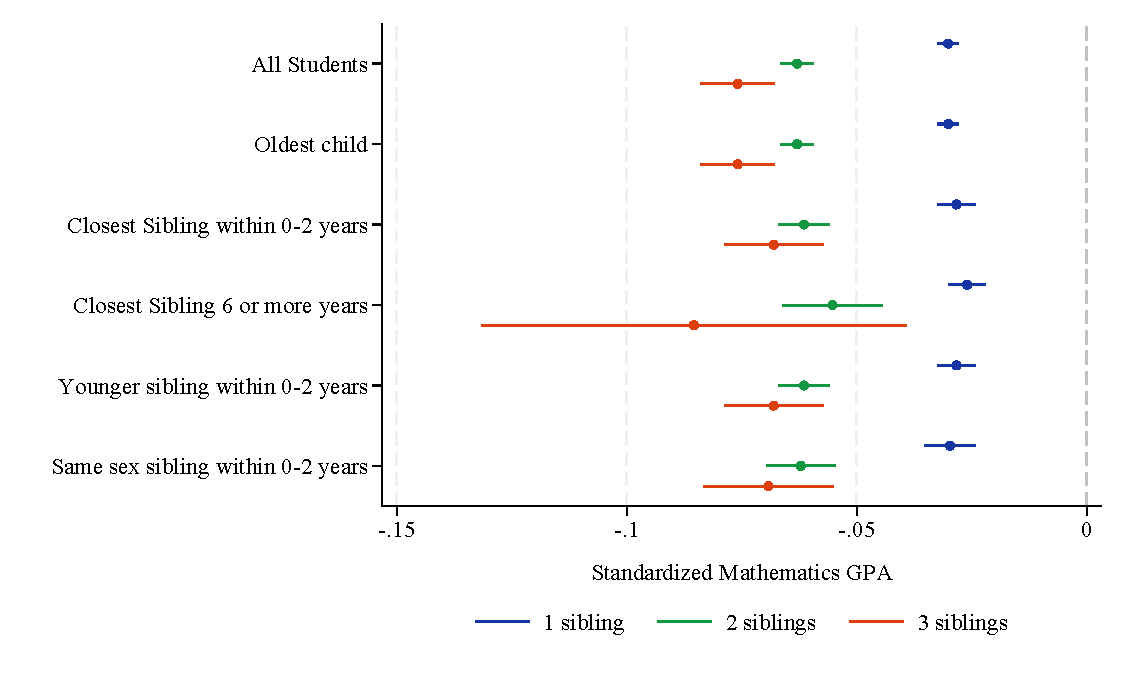
\includegraphics{./FIGURES/TWFE/covid_twfe_C_bysibs_elm_all_gpa_m_adj_Tsiblings_Soldest_4.pdf}
        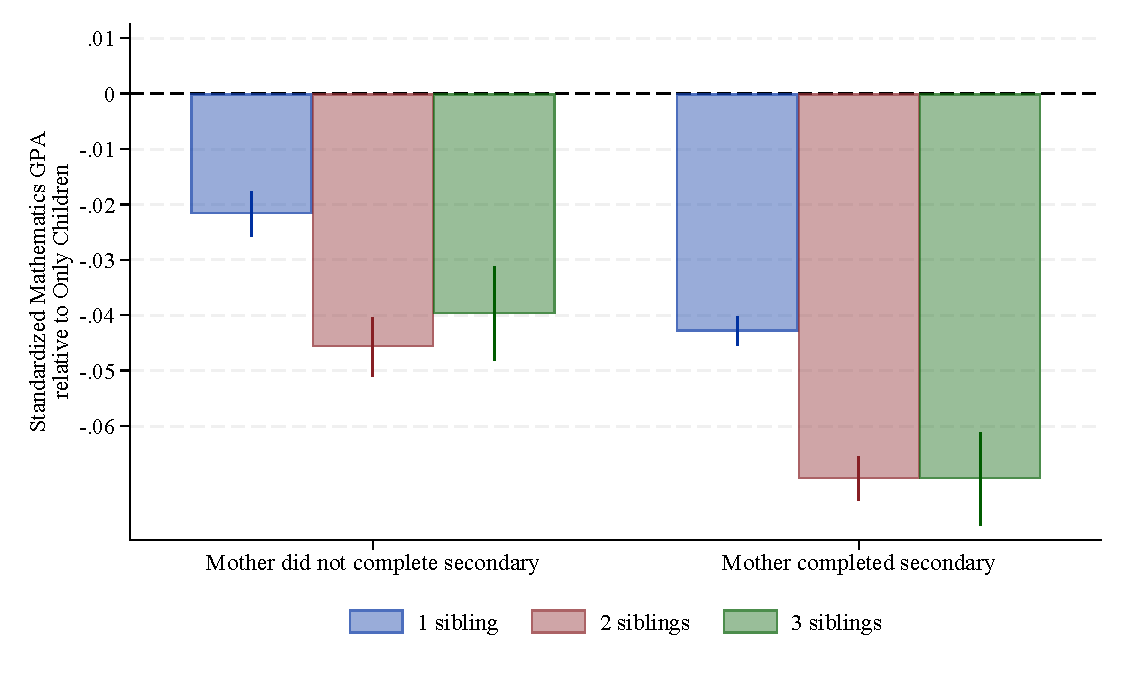
\includegraphics{./FIGURES/TWFE/twfe_gpa_mom_sec_complete_bysibs_20_21_Tsiblings_Soldest_4.pdf}
      }
    }

    \begin{flushleft}
        \hyperlink{frame:mothereduc}{\beamergotobutton{Go Back $\carriagereturn$}}
    \end{flushleft}        

\end{frame}

\begin{comment}
\begin{frame}
    \label{frame:livesmother}
    \frametitle{Lives with mother}
        {\resizebox{0.9\textwidth}{!}{
        %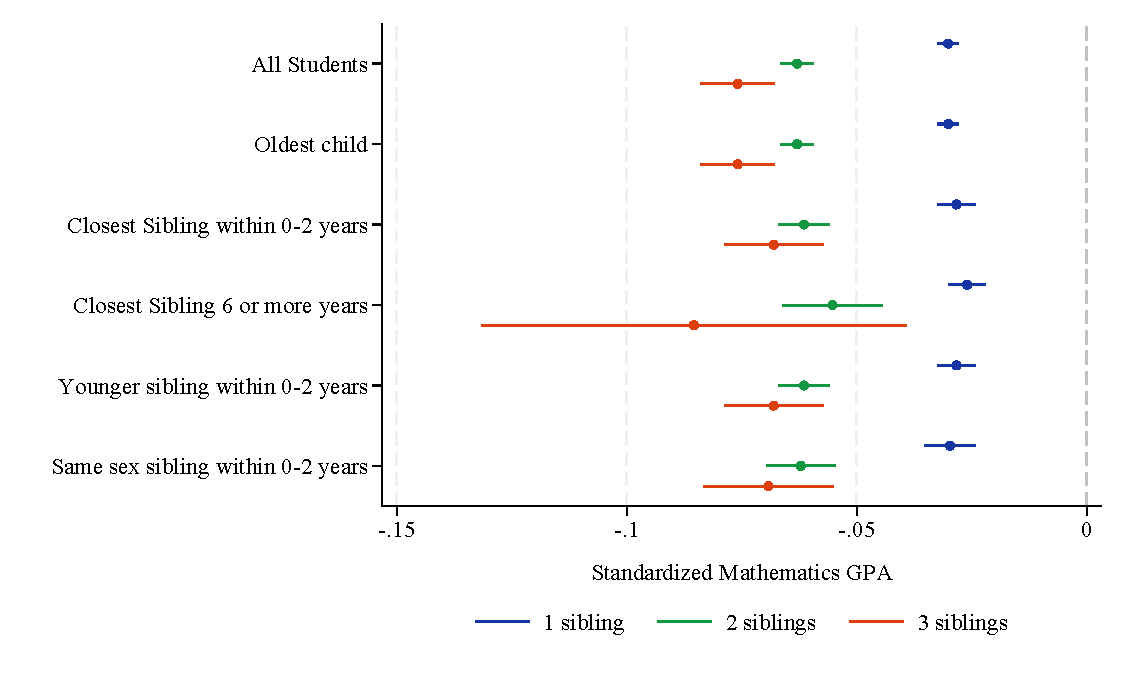
\includegraphics{./FIGURES/TWFE/covid_twfe_C_bysibs_elm_all_gpa_m_adj_Tsiblings_Soldest_4.pdf}
        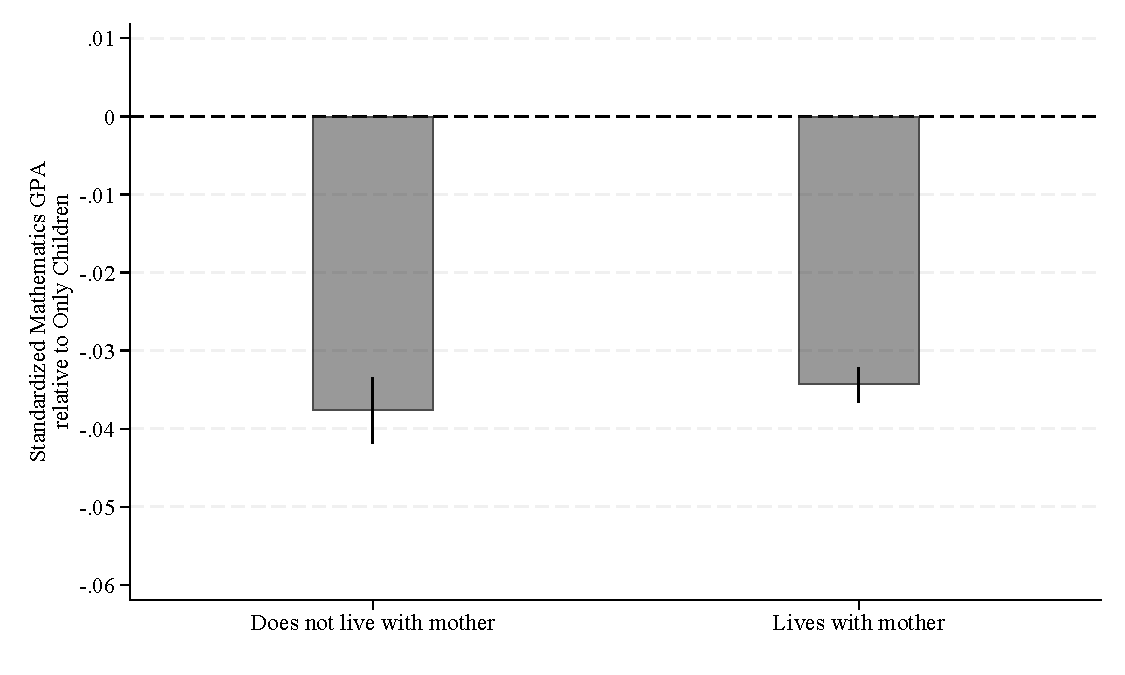
\includegraphics{./FIGURES/TWFE/twfe_gpa_lives_with_mother_20_21_Tsiblings_Soldest_4.pdf}
      }
    }

    \begin{flushleft}
        \hyperlink{frame:livesmother_siblings}{\beamergotobutton{Results by siblings}}
    \end{flushleft}    

\end{frame}

\begin{frame}
    \label{frame:livesmother_siblings}
    \frametitle{Lives with mother}
        {\resizebox{0.9\textwidth}{!}{
        %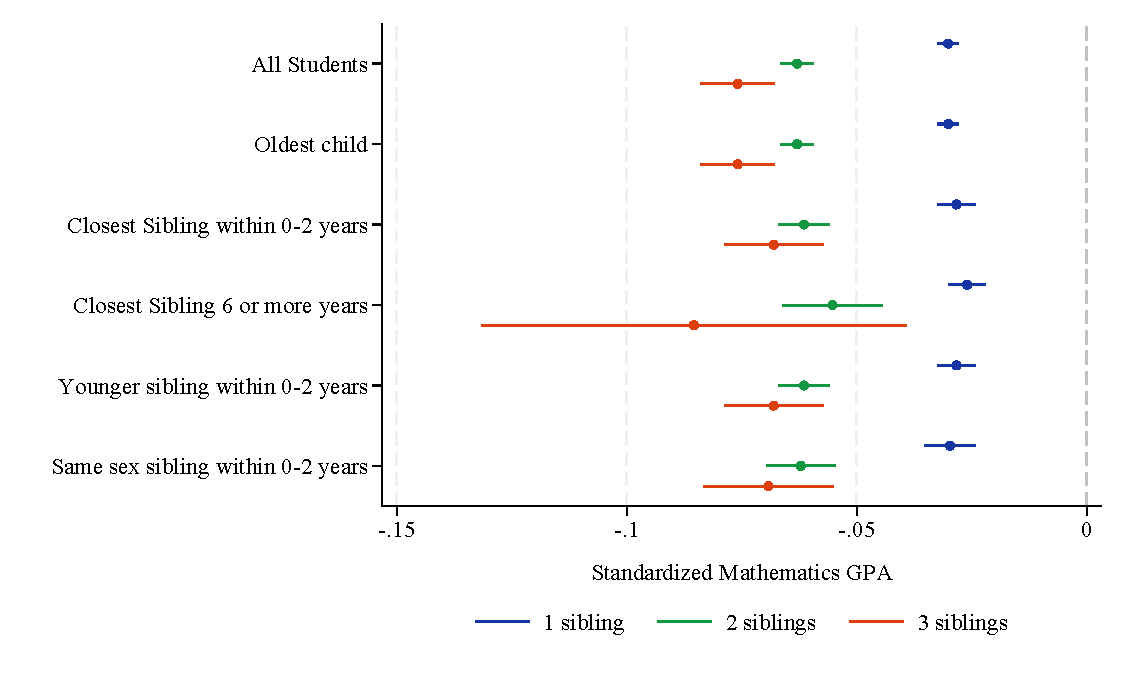
\includegraphics{./FIGURES/TWFE/covid_twfe_C_bysibs_elm_all_gpa_m_adj_Tsiblings_Soldest_4.pdf}
        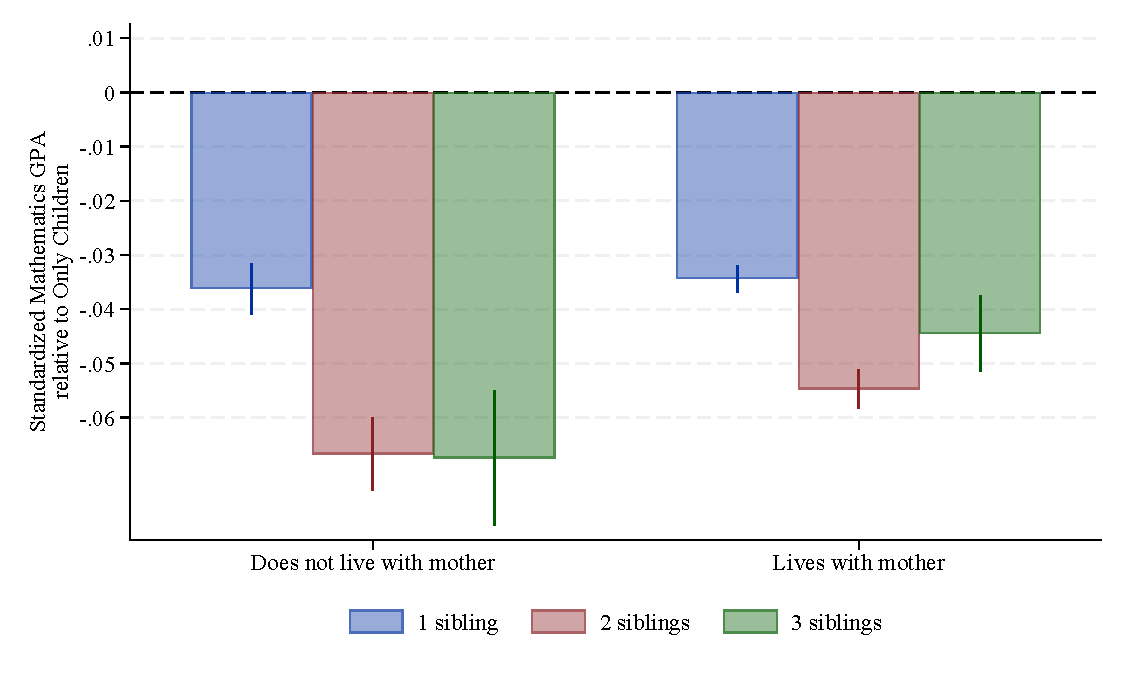
\includegraphics{./FIGURES/TWFE/twfe_gpa_lives_with_mother_bysibs_20_21_Tsiblings_Soldest_4.pdf}
      }
    }

    \begin{flushleft}
        \hyperlink{frame:livesmother}{\beamergotobutton{Go Back $\carriagereturn$}}
    \end{flushleft}        

\end{frame}
\end{comment}




\begin{frame}
    \label{frame:childcare}
    \frametitle{Parental dilution - Increased childcare}
       \begin{itemize}
            \item We use effects of delayed schooling (more childcare) outside of Covid to have a sense of how parents react to this.
            \item Mixed results in literature (US and Denmark) although not until younger starts school.
        \end{itemize}
\end{frame}      

\begin{frame}
    \label{frame:delayedentry}
    \frametitle{Effects of delaying younger School Entry (GPA of older)}
    \makeatletter
\@ifclassloaded{beamer}{%
       \centering
       \resizebox{0.6\textwidth}{!}%
}{%
       \begin{table}[!tbp]\centering\def\sym#1{\ifmmode^{#1}\else\(^{#1}\)\fi}
       \centering
       \caption{Effects of younger sibling delaying school on older sibling standardized exams - 1 - m - a -  - 365}
       \label{tab:rd_summ_1_m_a_365}
       \resizebox{0.95\textwidth}{!}%
}
{
\makeatother
\resizebox{\textwidth}{!}{
\begin{tabular}{lccc}
\toprule
\cmidrule(lr){2-4}
& \multicolumn{3}{c}{Standardized GPA} \\
\cmidrule(lr){2-4}
& Pre-Covid & Covid & Post-Covid  \\
& 2018-2019 & 2020-2021 & 2022-2023  \\
\cmidrule(lr){2-2} \cmidrule(lr){3-3} \cmidrule(lr){4-4}
& (1) & (2) & (3)  \\
\bottomrule
&  &  &   \\
\multirow{2}{*}{\shortstack[l]{Younger sibling born after \\ school-entry cutoff}}&      -0.023***&      -0.001   &      -0.023***\\
                    &     (0.007)   &     (0.007)   &     (0.006)   \\
Local Linear        &         Yes   &         Yes   &         Yes   \\
                    &               &               &               \\
Observations        &     358,861   &     354,044   &     447,536   \\
Counterfactual mean &       0.058   &       0.020   &       0.050   \\
Bandwidth           &         365   &         365   &         365   \\
 

\bottomrule
\end{tabular}
}
\@ifclassloaded{beamer}{%
}{%
       \end{table}
}


      
    \only<2->{
    \highlightboxflex{-0.6}{-0.2}{1.2}{1.0}{draw=blue, draw opacity=0.8, dashed, fill=yellow!30, fill opacity=0.3}
    
    % Highlight box for Covid same sex coefficient  
    \highlightboxflex{1.85}{-0.2}{1.2}{1.0}{draw=blue, draw opacity=0.8, dashed, fill=yellow!30, fill opacity=0.3}
    
    \begin{tikzpicture}[overlay, remember picture]
        % Single text label at the bottom
        \node[red, above] at ([shift={(0,-2.8)}]current page.center) {\small Negative spillover of having a younger sibling stay at home};
        
        % Arrow to Pre-Covid coefficient (pointing to the left box)
        \draw[->, thick, blue, opacity=0.4] ([shift={(0,-2.2)}]current page.center) -- ([shift={(-0.6,-0.25)}]current page.center);
        
        % Arrow to Covid coefficient (pointing to the right box)
        \draw[->, thick, blue, opacity=0.4] ([shift={(0,-2.2)}]current page.center) -- ([shift={(1.85,-0.25)}]current page.center);
    \end{tikzpicture}
    }
\end{frame}

\begin{frame}
    \label{frame:delayedentryscores}
    \frametitle{Effects of delaying younger School Entry (Scores and investment)}
\makeatletter
     \centering
       \resizebox{0.95\textwidth}{!}%
{
\makeatother
\begin{tabular}{lccccc}
\toprule
& \multicolumn{2}{c}{Pre-Covid}  & \multicolumn{3}{c}{Post-Covid} \\
& \multicolumn{2}{c}{2018-2019}  & \multicolumn{3}{c}{2022-2024}  \\
\cmidrule(lr){2-3} \cmidrule(lr){4-6}
& Mathematics & Reading & Mathematics & Reading & Parental Time Investment  \\
& (1) & (2) & (3) & (4) & (5) \\
\bottomrule
&  &  &  & &  \\
\multirow{2}{*}{\shortstack[l]{Younger sibling born after \\ school-entry cutoff}}&      -0.025*  &      -0.023*  &      -0.009   &      -0.012   &      -0.035***\\
                    &     (0.014)   &     (0.012)   &     (0.013)   &     (0.010)   &     (0.013)   \\
Local Linear        &         Yes   &         Yes   &         Yes   &         Yes   &         Yes   \\
                    &               &               &               &               &               \\
Observations        &      86,605   &      86,602   &     104,983   &     105,064   &     101,766   \\
Counterfactual mean &      -0.105   &      -0.083   &       0.194   &       0.288   &      -0.004   \\
Bandwidth           &         365   &         365   &         365   &         365   &         365   \\
 

\bottomrule
\end{tabular}
}

    \only<2->{

    % Highlight box for Covid same sex coefficient  
    \highlightboxflex{3.20}{-0.77}{1.2}{1.0}{draw=blue, draw opacity=0.8, dashed, fill=yellow!30, fill opacity=0.3}
    
    \begin{tikzpicture}[overlay, remember picture]
        % Single text label at the bottom
        \node[red, above] at ([shift={(0,-2.8)}]current page.center) {\small Reduce parental time investment when younger sibling stays at home};

  
        
        % Arrow to Covid coefficient (pointing to the right box)
        \draw[->, thick, blue, opacity=0.4] ([shift={(0,-2.2)}]current page.center) -- ([shift={(3.20,-0.77)}]current page.center);
    \end{tikzpicture}
    }

\end{frame}

\begin{frame}
    \label{frame:incomeshocks}
    \frametitle{Income Shocks}
     
    %\makeatletter
\@ifclassloaded{beamer}{%
       \centering
       \resizebox{0.6\textwidth}{!}%
}{%
       \begin{table}[!tbp]\centering\def\sym#1{\ifmmode^{#1}\else\(^{#1}\)\fi}
       \centering
       \caption{TWFE on Standardized Exams, Expectations and Socio-Economic Status}
       \label{tab:twfe_ece}
       \resizebox{0.8\textwidth}{!}%
}
{
\makeatother
\begin{tabular}{lccc}
\toprule
\cmidrule(lr){2-4}
& \multicolumn{3}{c}{TWFE}  \\
\cmidrule(lr){2-4}
& 1 sibling & 2 siblings & 3 siblings  \\
\cmidrule(lr){2-2} \cmidrule(lr){3-3} \cmidrule(lr){4-4}
& (1) & (2) & (3)\\
\bottomrule
&  &  &  \\
&  &  &   \\
\multicolumn{4}{l}{\textit{Panel A: 2nd grade students}} \\
\hspace{3mm}Mathematics&      -0.028** &      -0.090***&      -0.093   \\
                    &     (0.011)   &     (0.023)   &     (0.081)   \\
 
%&  &  &   \\
\hspace{3mm}Reading &      -0.028** &      -0.068***&      -0.140*  \\
                    &     (0.011)   &     (0.022)   &     (0.078)   \\
 
%&  &  &   \\
\hspace{3mm}Max Expectation: Finish school&       0.008***&      -0.002   &      -0.026   \\
                    &     (0.003)   &     (0.006)   &     (0.022)   \\
 
%&  &  &   \\
\hspace{3mm}Max Expectation: 4-year college&      -0.011** &       0.004   &      -0.010   \\
                    &     (0.004)   &     (0.009)   &     (0.034)   \\
 
%&  &  &   \\
\hspace{3mm}SES     &       0.018** &       0.022   &       0.058   \\
                    &     (0.009)   &     (0.019)   &     (0.069)   \\
 
&  &  &   \\
\multicolumn{4}{l}{\textit{Panel B: 4th grade students}} \\
\hspace{3mm}Mathematics&      -0.022***&      -0.103***&      -0.172***\\
                    &     (0.004)   &     (0.008)   &     (0.022)   \\
 
%&  &  &   \\
\hspace{3mm}Reading &      -0.027***&      -0.103***&      -0.139***\\
                    &     (0.004)   &     (0.008)   &     (0.022)   \\
 
%&  &  &   \\
\hspace{3mm}Max Expectation: Finish school&       0.006***&       0.004   &       0.005   \\
                    &     (0.001)   &     (0.003)   &     (0.008)   \\
 
%&  &  &   \\
\hspace{3mm}Max Expectation: 4-year college&      -0.012***&      -0.020***&      -0.032***\\
                    &     (0.002)   &     (0.004)   &     (0.010)   \\
 
%&  &  &   \\
\hspace{3mm}SES     &       0.017***&      -0.005   &       0.004   \\
                    &     (0.003)   &     (0.006)   &     (0.019)   \\
 
&  &  &   \\
\multicolumn{4}{l}{\textit{Panel C: 8th grade students}} \\
\hspace{3mm}Mathematics&      -0.014** &      -0.036***&      -0.029   \\
                    &     (0.007)   &     (0.010)   &     (0.018)   \\
 
%&  &  &   \\
\hspace{3mm}Reading &       0.005   &      -0.009   &      -0.023   \\
                    &     (0.007)   &     (0.009)   &     (0.017)   \\
 
%&  &  &   \\
\hspace{3mm}Max Expectation: Finish school&      -0.011   &      -0.001   &       0.051***\\
                    &     (0.010)   &     (0.013)   &     (0.019)   \\
 
%&  &  &   \\
\hspace{3mm}Max Expectation: 4-year college&      -0.007   &      -0.003   &      -0.054** \\
                    &     (0.014)   &     (0.017)   &     (0.026)   \\
 
%&  &  &   \\
\hspace{3mm}SES     &       0.017***&       0.026***&       0.038***\\
                    &     (0.005)   &     (0.008)   &     (0.014)   \\
 

\bottomrule
\end{tabular}
}
\@ifclassloaded{beamer}{%
}{%
       \end{table}
}


     {\resizebox{0.9\textwidth}{!}{
        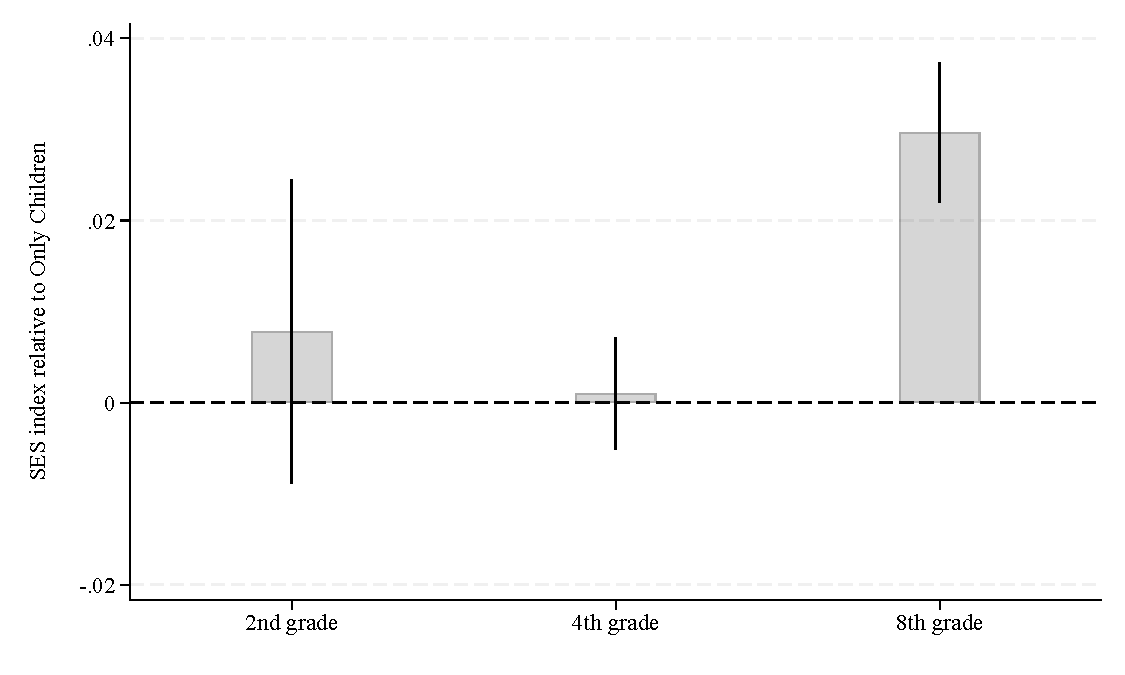
\includegraphics{./FIGURES/TWFE/twfe_ses_2_4_8_Tsiblings_Soldest_4.pdf}
      }
    }
\end{frame}



\begin{frame}
    \label{frame:iv_intro}
    \frametitle{Effect of family size on GPA: Using Same Sex and Twin IV}
    \begin{itemize}
        \item To address any further remaining endogeneity concerns such as time-varying unobserved shocks we use an IV approach.
        \item Having same sex children (BB or GG) makes families more likely to have a third child. Twin births is also used as a potential exogenous variation in family size.
    \end{itemize}    
   
\end{frame}

\begin{frame}[t]
    \label{frame:iv_results}
    \frametitle{Effect of family size on GPA: Using same sex and twin births IV}
    \begin{table}[h]
\centering
\caption{Effect of Family Size on GPA}
\label{tab:twfe_twins}
\resizebox{0.95\textwidth}{!}{%
\begin{tabular}{lHccccHcccc}
\hline
& \multicolumn{5}{c}{Pre-Covid} & \multicolumn{5}{c}{Covid (2020-2021)} \\
\cmidrule(lr){2-6} \cmidrule(lr){7-11}
& OLS & OLS & First & Second & N & OLS & OLS & First & Second & N \\
& (no controls) & (controls) & Stage & Stage & & (no controls) & (controls) & Stage & Stage & \\
\hline
& & & & & & & & & & \\
Instrument: first two children same sex & & & 0.050* & & 3,300,349 & & & 0.047* & & 2,809,126 \\
\quad (Sample: first and second children in families & & & (0.001) & & & & & (0.001) & & \\
\quad with two or more births) & & & & & & & & & & \\
Number of children in family & $-0.081$* & $-0.070$* & & 0.063* & & $-0.119$* & $-0.101$* & & $-0.031$ & \\
& (0.001) & (0.001) & & (0.022) & & (0.001) & (0.001) & & (0.025) & \\
Instrument: twin at second birth & & & 0.813* & & 1,589,159 & & & 0.855* & & 1,240,864 \\
\quad (Sample: First child in families with two or more & & & (0.006) & & & & & (0.006) & & \\
\quad births) & & & & & & & & & & \\
Number of children in family & $-0.090$* & $-0.056$* & & 0.012 & & $-0.125$* & $-0.085$* & & 0.009 & \\
& (0.001) & (0.001) & & (0.012) & & (0.002) & (0.002) & & (0.013) & \\
& & & & & & & & & & \\
%Instrument: twin at third birth & & & 0.819* & & 1,195,717 & & & 0.866* & & 841,770 \\
%\quad (Sample: first and second children in families & & & (0.006) & & & & & (0.006) & & \\
%\quad with three or more births) & & & & & & & & & & \\
%Number of children in family & $-0.104$* & $-0.090$* & & $-0.020$ & & $-0.118$* & $-0.101$* & & $-0.019$ & \\
%& (0.002) & (0.002) & & (0.013) & & (0.002) & (0.002) & & (0.014) & \\
%& & & & & & & & & & \\
\hline
\end{tabular}%
}
\end{table}
   
    \only<2->{
    \highlightboxflex{0.3}{-0.25}{0.8}{0.7}{draw=blue, draw opacity=0.8, dashed, fill=yellow!30, fill opacity=0.3}
    
    % Highlight box for Covid same sex coefficient  
    \highlightboxflex{3.55}{-0.25}{0.8}{0.7}{draw=blue, draw opacity=0.8, dashed, fill=yellow!30, fill opacity=0.3}
    
    \begin{tikzpicture}[overlay, remember picture]
        % Single text label at the bottom
        \node[red, above] at ([shift={(0,-2.8)}]current page.center) {\small Reduction in family size effect!};
        
        % Arrow to Pre-Covid coefficient (pointing to the left box)
        \draw[->, thick, blue, opacity=0.4] ([shift={(0,-2.2)}]current page.center) -- ([shift={(0.3,-0.25)}]current page.center);
        
        % Arrow to Covid coefficient (pointing to the right box)
        \draw[->, thick, blue, opacity=0.4] ([shift={(0,-2.2)}]current page.center) -- ([shift={(3.55,-0.25)}]current page.center);
    \end{tikzpicture}
    }
\end{frame}

\begin{frame}
    \label{frame:iv_conclusion}
    \frametitle{Effect of family size on GPA: Using Same Sex and Twin IV}
 \begin{itemize}
        \item We see a negative reduction in family size effects on performance using same sex IV.
        \item Twin IV might not be well suited for this context. Parents may be more able to teach, study and help siblings that share coursework. 
        %\item One reason why we don't find results could be that to some this captures more the effect of monetary cost but in terms of time, twins might not be twice as costly than two separate children
        \item We are estimating here the differential effect from \#2 to \#3.
    \end{itemize}
\end{frame}

% ========================================
% BEYOND PERFORMANCE
% ========================================
\section{Beyond performance}

    \begin{frame}
            \label{frame:expectations}
            \frametitle{Reduction in educational expectations}
      {\resizebox{0.9\textwidth}{!}{
        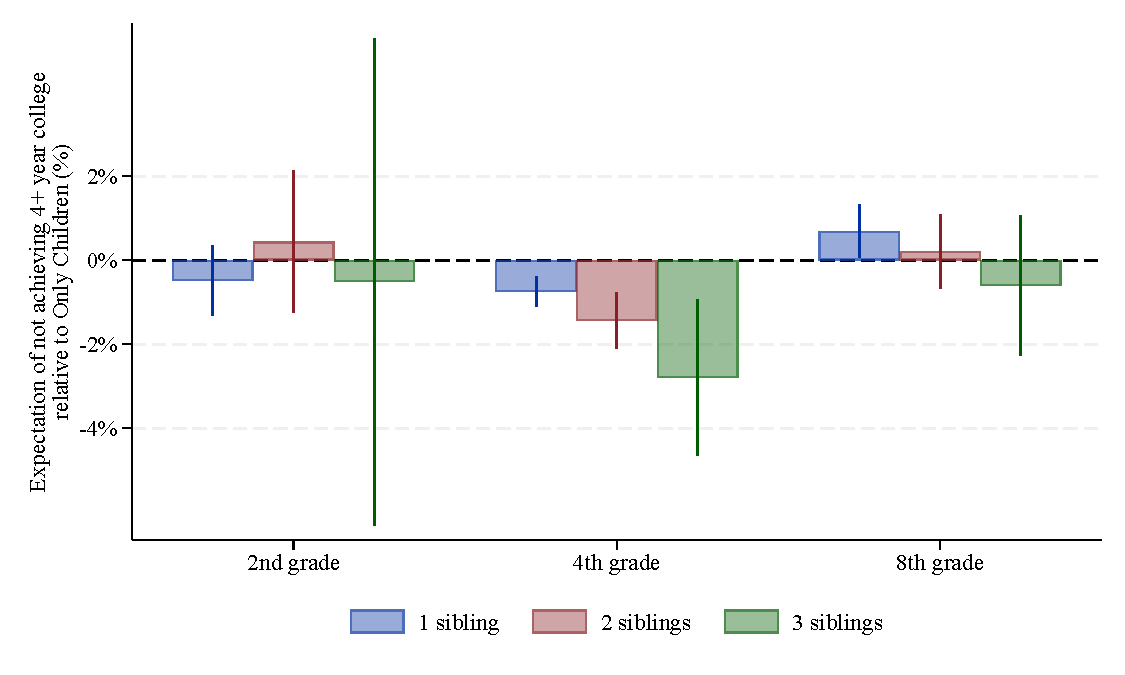
\includegraphics{./FIGURES/TWFE/twfe_expectation_bysibs_2_4_8_Tsiblings_Soldest_4.pdf}
      }
    }   %\input{./TABLES/MANUAL/twfe_ece_expectations.tex}
    \end{frame}

    \begin{frame}
            \label{frame:grade_progression}
            \frametitle{Grade progression}
    %\input{./TABLES/MANUAL/twfe_ece_expectations.tex}
    \end{frame}   

    \begin{frame}
            \label{frame:college_app}
            \frametitle{College Applications}
    %\input{./TABLES/MANUAL/twfe_ece_expectations.tex}
    \end{frame}      

% ========================================
% EXTERNAL VALIDITY
% ========================================
\section{External Validity}

    \begin{frame}
            \label{frame:pisadata}
            \frametitle{Is this only about Peru?}
        \begin{itemize}
            \item International examination to 15 year olds
            \item 81 countries (37 OECD and 44 non-OECD).
            \item In 2009, 2012 and 2022, I am able to identify only-child and sibling sample.
            \item In most countries, children with siblings also exhibit larger learning losses
            \item Longer school closures where associated with larger gaps.
        \end{itemize}
    \end{frame}

\begin{frame}
    \label{frame:pisagaps}
    \frametitle{Learning gaps in Mathematics by year}
    
    \begin{figure}
        \centering
        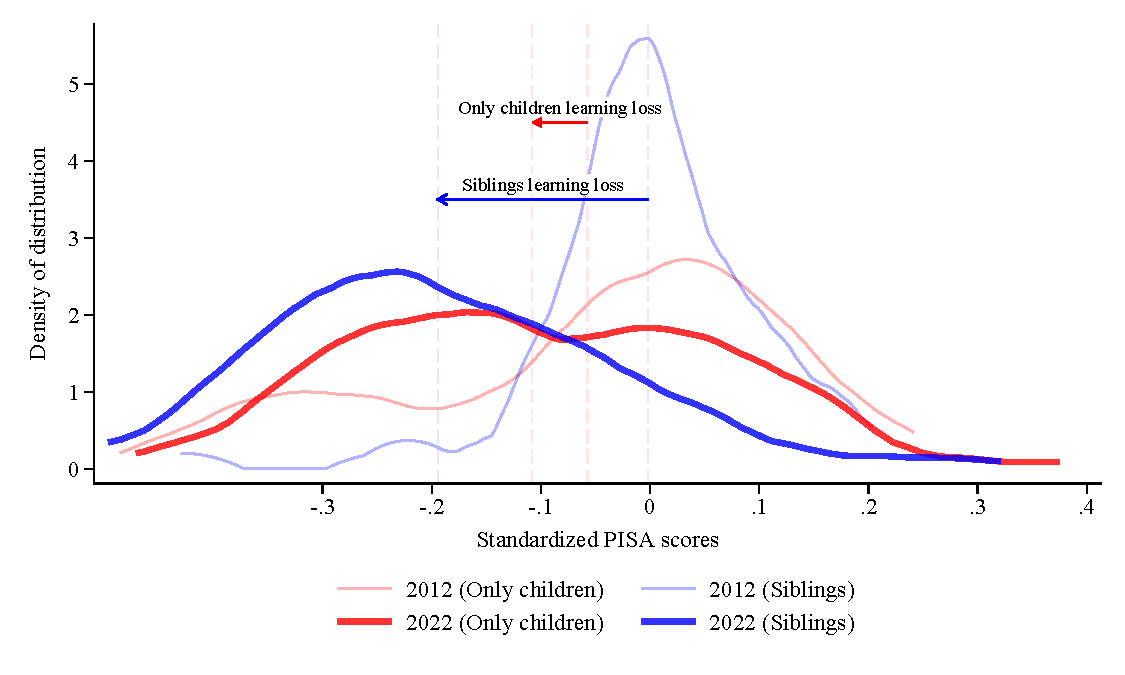
\includegraphics[width=0.9\textwidth]{./FIGURES/Descriptive/PISA_distribution_2012_2022_PV4MATH.pdf}
        \caption{Learning gaps in Mathematics by year}
        \label{fig:1a}
    \end{figure}
    
\end{frame}

\begin{frame}
    \label{frame:pisaclosure}
    \frametitle{Change in learning gaps by duration of school closure}
    
    \begin{figure}
        \centering
        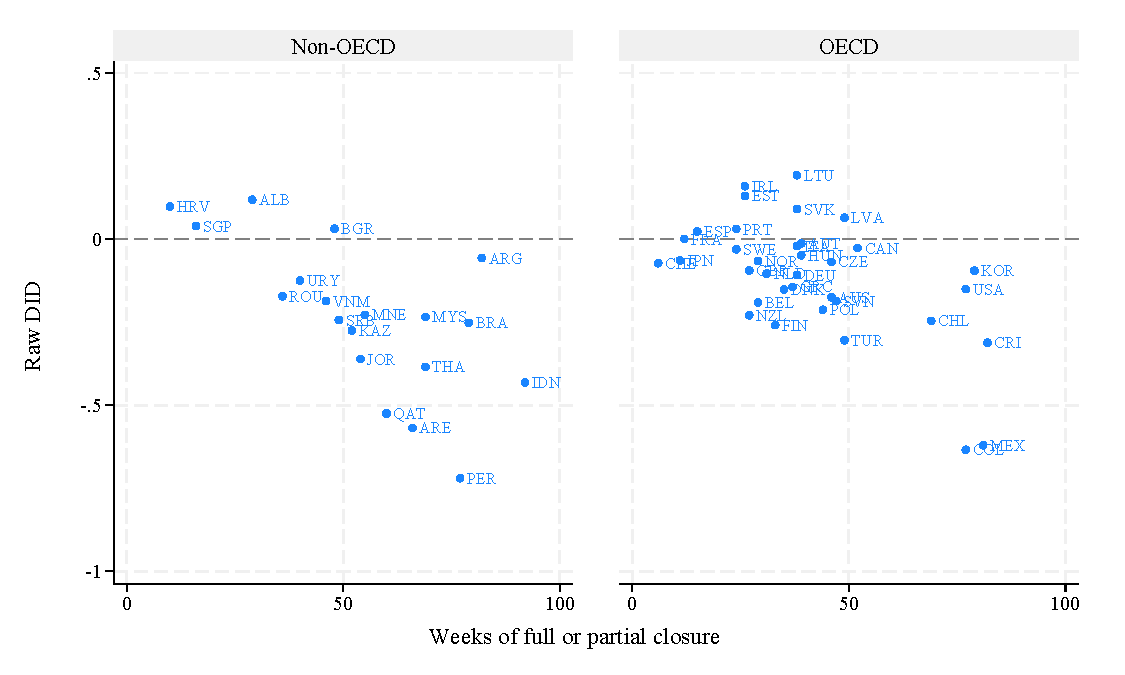
\includegraphics[width=0.9\textwidth]{./FIGURES/Descriptive/PISA_raw_DID_PV4MATH_not_fully_open.pdf}
        \caption{Similar pattern in rest of the world}
        \label{fig:1b}
    \end{figure}
    
    
\end{frame}





% ========================================
% CONCLUSIONS
% ========================================
\section{Conclusions}

\begin{frame}
    \label{frame:conclusions}
    \frametitle{Conclusions}
    \begin{itemize}
        \item Should crisis interventions differentiate by family structure?
        \item Does resource stress activate latent quantity-quality tradeoffs in family investment?
    \end{itemize}


\end{frame}


\begin{frame}
    \hypersetup{citecolor=blue}
  \centering
  \vspace{2cm}
  {\Huge \textbf{Thank you!}} \\[1cm]
  
  {\Large Questions or comments?} \\[0.5cm]
  
  \rule{0.4\linewidth}{0.4pt} \\[0.5cm]
  
  \begin{flushleft}
    \textbf{Francisco Pardo} \\
    University of Texas at Austin \\
    fpardo@utexas.edu \\
    %\href{mailto:fpardo@utexas.edu}{fpardo@utexas.edu} \\
    \href{https://francisco-pardo-pajuelo.github.io/}{Website}
  \end{flushleft}

\end{frame}

% ========================================
% EXAMPLE SLIDES
% ========================================
\section{Example Slides}





\begin{frame}[allowframebreaks]
    \frametitle{References}
    \small
    \tiny\bibliography{references}  % <- Call your .bib file here (no .bib extension)
\end{frame}


% ========================================
% NAVIGATION SLIDE - COMPACT VERSION
% ========================================
\begin{frame}
    \label{frame:navigation}
    \frametitle{Presentation Navigation}
    
    \small % Reduce overall font size
    
    \begin{columns}[T]
        \begin{column}{0.45\textwidth}
            \centering
            \textbf{Introduction \& Setup}
            \vspace{0.1cm}
            
            \hyperlink{frame:motivation}{\beamergotobutton{Motivation}}\\[2pt]
            \hyperlink{frame:thispaper}{\beamergotobutton{This Paper}}\\[2pt]
            \hyperlink{frame:contribution}{\beamergotobutton{Literature}}\\[2pt]
            \hyperlink{frame:background}{\beamergotobutton{Background}}\\[2pt]
            \hyperlink{frame:data}{\beamergotobutton{Data}}\\[2pt]
            \hyperlink{frame:trends}{\beamergotobutton{Data Trends}}
            
            \vspace{0.2cm}
            \textbf{Mechanisms}
            \vspace{0.1cm}
            
            \hyperlink{frame:mechanisms}{\beamergotobutton{Potential Mechanisms}}\\[2pt]
            \hyperlink{frame:birthorder}{\beamergotobutton{Birth Order}}\\[2pt]
            \hyperlink{frame:ses}{\beamergotobutton{SES Analysis}}\\[2pt]
            \hyperlink{frame:pcinternet}{\beamergotobutton{PC \& Internet}}\\[2pt]
            \hyperlink{frame:siblingdisruption}{\beamergotobutton{Sibling Disruption}}\\[2pt]
            \hyperlink{frame:parentaldilution}{\beamergotobutton{Parental Dilution}}
        \end{column}
        
        \begin{column}{0.45\textwidth}
            \centering
            \textbf{Methodology \& Results}
            \vspace{0.1cm}
            
            \hyperlink{frame:research}{\beamergotobutton{Research Design}}\\[2pt]
            \hyperlink{frame:empirical}{\beamergotobutton{Empirical Strategy}}\\[2pt]
            \hyperlink{frame:eventstudy}{\beamergotobutton{Event Study}}\\[2pt]
            \hyperlink{frame:twfe}{\beamergotobutton{TWFE Results}}\\[2pt]
            \hyperlink{frame:twfeexams}{\beamergotobutton{Standardized Exams}}
            
            \vspace{0.2cm}
            \textbf{Additional Analysis}
            \vspace{0.1cm}
            
            \hyperlink{frame:childcare}{\beamergotobutton{Childcare Effects}}\\[2pt]
            \hyperlink{frame:delayedentry}{\beamergotobutton{Delayed Entry}}\\[2pt]
            \hyperlink{frame:incomeshocks}{\beamergotobutton{Income Shocks}}\\[2pt]
            \hyperlink{frame:otherstrategies}{\beamergotobutton{Other Strategies}}\\[2pt]
            \hyperlink{frame:twiniv}{\beamergotobutton{Twin IV}} \\[2pt]
            \hyperlink{frame:expectations}{\beamergotobutton{Expectations}}
            
        \end{column}
    \end{columns}
    
    \vspace{0.2cm}
    
    \begin{center}
        \textbf{External Validity \& Conclusions}\\[4pt]
        \hyperlink{frame:pisadata}{\beamergotobutton{PISA Data}} \quad
        \hyperlink{frame:pisagaps}{\beamergotobutton{Learning Gaps}} \quad
        \hyperlink{frame:pisaclosure}{\beamergotobutton{School Closure}} \quad
        \hyperlink{frame:conclusions}{\beamergotobutton{Conclusions}}
    \end{center}
\end{frame}


\begin{frame}
    \label{frame:highlightfigure}
    \frametitle{Highlighting Parts of slide}
    \highlightboxflex{-3.5}{0.5}{1.5}{1.5}{draw=blue, draw opacity=0.8, dashed, fill=yellow!30, fill opacity=0.3}
    \begin{tikzpicture}[overlay, remember picture]
        \node[red, above] at ([shift={(-2.75,2.2)}]current page.center) {\small Key finding!};
        \draw[->, thick, blue, opacity=0.8] ([shift={(-2.5,-2.5)}]current page.center) -- ([shift={(-3.1,0.5)}]current page.center);
%blue!50!black
    \end{tikzpicture}
\end{frame}


\begin{frame}
    \label{frame:research_feedback}
    \frametitle{Threats to identification \textcolor{red}{(for feedback)}}
        Any other thoughts on potential time varying shocks?
        \begin{itemize}
            \item Parent's work
            \item 
            \item There is a shift from private to public enrollment during COVID. If this was more common on siblings... would be composition?
        \end{itemize}
\end{frame}


\begin{frame}
    \label{frame:twfe}
    \frametitle{TWFE results}
        {\resizebox{0.9\textwidth}{!}{
       %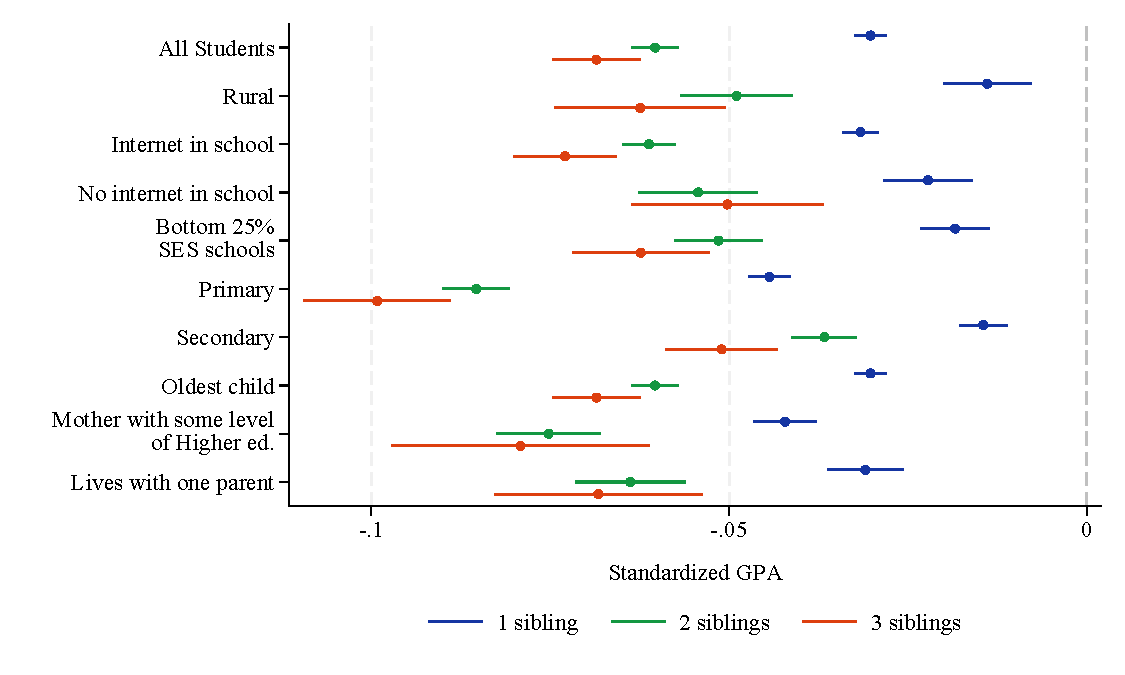
\includegraphics{./FIGURES/TWFE/covid_twfe_summ_bysibs_all_20-21_gpa_m_adj_Tsiblings_Soldest_4.pdf}
       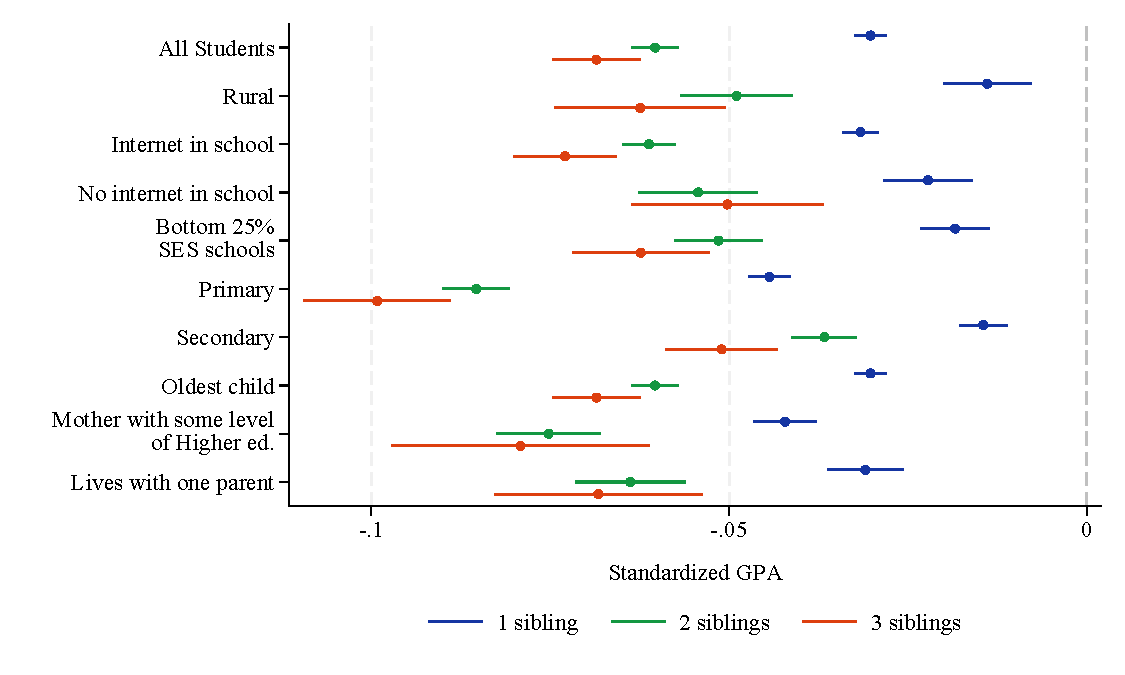
\includegraphics{./FIGURES/TWFE/covid_twfe_summ_bysibs_all_20-21_gpa_m_adj_Tsiblings_Soldest_4.pdf}
      }
    }
\end{frame}


\begin{frame}
\label{frame:twfeexams}
\frametitle{TWFE - Standardized Exams}
       \centering
       \resizebox{0.7\textwidth}{!}%
{
\makeatother
\begin{tabular}{lcccc}
\toprule
\cmidrule(lr){2-5}
& \multicolumn{4}{c}{TWFE} \\
\cmidrule(lr){2-5}
& 1-3 siblings & 1 sibling & 2 siblings & 3 siblings  \\
\cmidrule(lr){2-2} \cmidrule(lr){3-3} \cmidrule(lr){4-4} \cmidrule(lr){5-5}
& (1) & (2) & (3) & (4) \\
\bottomrule
&  &  & &  \\
&  &  & &  \\
\multicolumn{5}{l}{Panel A: GPA } \\
Mathematics         &      -0.099***&      -0.011   &      -0.036***&      -0.059***\\
                    &     (0.009)   &     (0.009)   &     (0.011)   &     (0.015)   \\
                    &               &               &               &               \\ 
&  &  & &  \\
Reading             &      -0.099***&      -0.010   &      -0.031***&      -0.034** \\
                    &     (0.009)   &     (0.009)   &     (0.010)   &     (0.015)   \\
                    &               &               &               &               \\
Observations        &     326,669   &     280,846   &     225,840   &     180,218   \\
 
&  &  & &  \\
\multicolumn{5}{l}{Panel B: Standardized Exams } \\
Mathematics         &      -0.034***&      -0.017** &      -0.044***&      -0.071***\\
                    &     (0.006)   &     (0.007)   &     (0.008)   &     (0.011)   \\
                    &               &               &               &               \\ 
&  &  & &  \\
Reading             &      -0.013** &       0.002   &      -0.022***&      -0.046***\\
                    &     (0.006)   &     (0.006)   &     (0.008)   &     (0.011)   \\
                    &               &               &               &               \\
Observations        &     409,690   &     282,769   &     227,486   &     181,466   \\
 

\bottomrule
\end{tabular}
}

\end{frame}


\begin{frame}
    \label{frame:ses}
    \frametitle{Scarce material resources: Socio Economic Status}
       \centering
       \resizebox{0.7\textwidth}{!}{
\makeatother
\begin{tabular}{lcccc}
\toprule
\cmidrule(lr){2-5}
& \multicolumn{4}{c}{TWFE} \\
\cmidrule(lr){2-5}
& 1-3 siblings & 1 sibling & 2 siblings & 3 siblings  \\
\cmidrule(lr){2-2} \cmidrule(lr){3-3} \cmidrule(lr){4-4} \cmidrule(lr){5-5}
& (1) & (2) & (3) & (4) \\
\bottomrule
&  &  & &  \\
&  &  & &  \\

\multicolumn{5}{l}{Panel B: Low SES Households (Q1)} \\
Mathematics         &      -0.028***&      -0.009   &      -0.036***&      -0.061***\\
                    &     (0.005)   &     (0.006)   &     (0.006)   &     (0.008)   \\
 
&  &  & &  \\
Reading             &      -0.022***&      -0.010   &      -0.029***&      -0.044***\\
                    &     (0.005)   &     (0.006)   &     (0.007)   &     (0.008)   \\
                    &               &               &               &               \\
Observations        &     643,621   &     398,084   &     358,488   &     290,244   \\
 
&  &  & &  \\
\multicolumn{5}{l}{Panel C: High SES Households (Q4)} \\
Mathematics         &      -0.035***&      -0.029***&      -0.051***&      -0.072***\\
                    &     (0.006)   &     (0.007)   &     (0.009)   &     (0.019)   \\
 
&  &  & &  \\
Reading             &      -0.039***&      -0.032***&      -0.068***&      -0.010   \\
                    &     (0.006)   &     (0.007)   &     (0.010)   &     (0.019)   \\
                    &               &               &               &               \\
Observations        &     385,616   &     318,633   &     230,174   &     186,296   \\
 

\bottomrule
\end{tabular}
}

\end{frame}



\begin{transitionframe}
    \label{frame:parentaldilution}
    \frametitle{Parental dilution}
        {\resizebox{0.9\textwidth}{!}{
        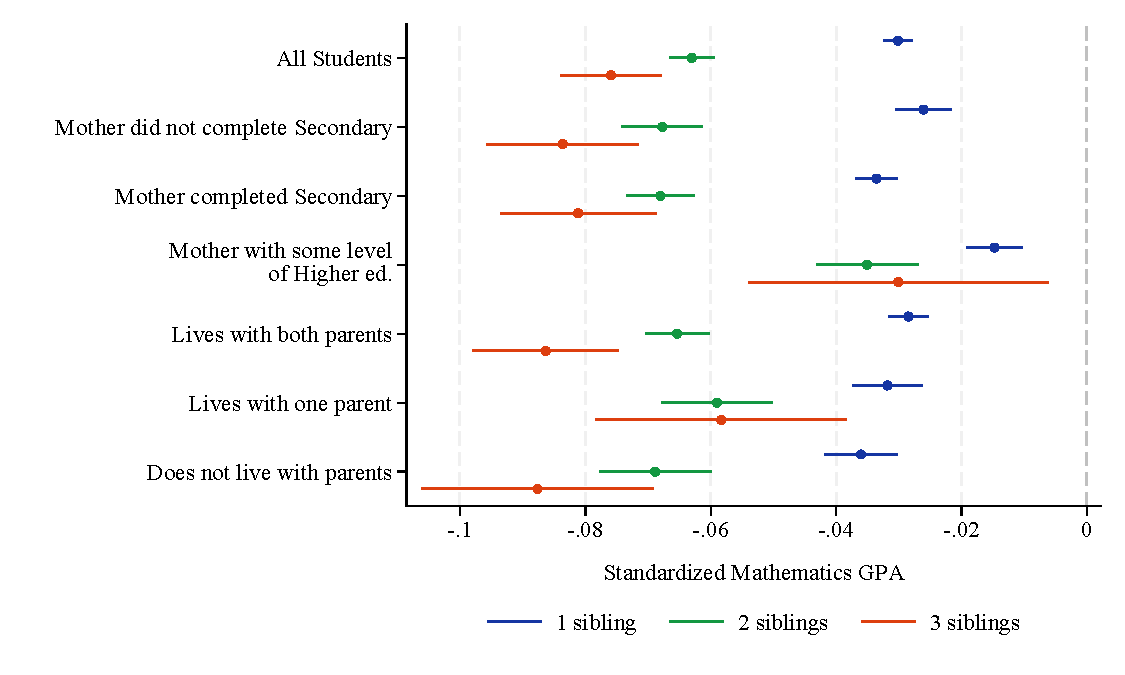
\includegraphics{./FIGURES/TWFE/covid_twfe_D_bysibs_elm_all_gpa_m_adj_Tsiblings_Soldest_4.pdf}%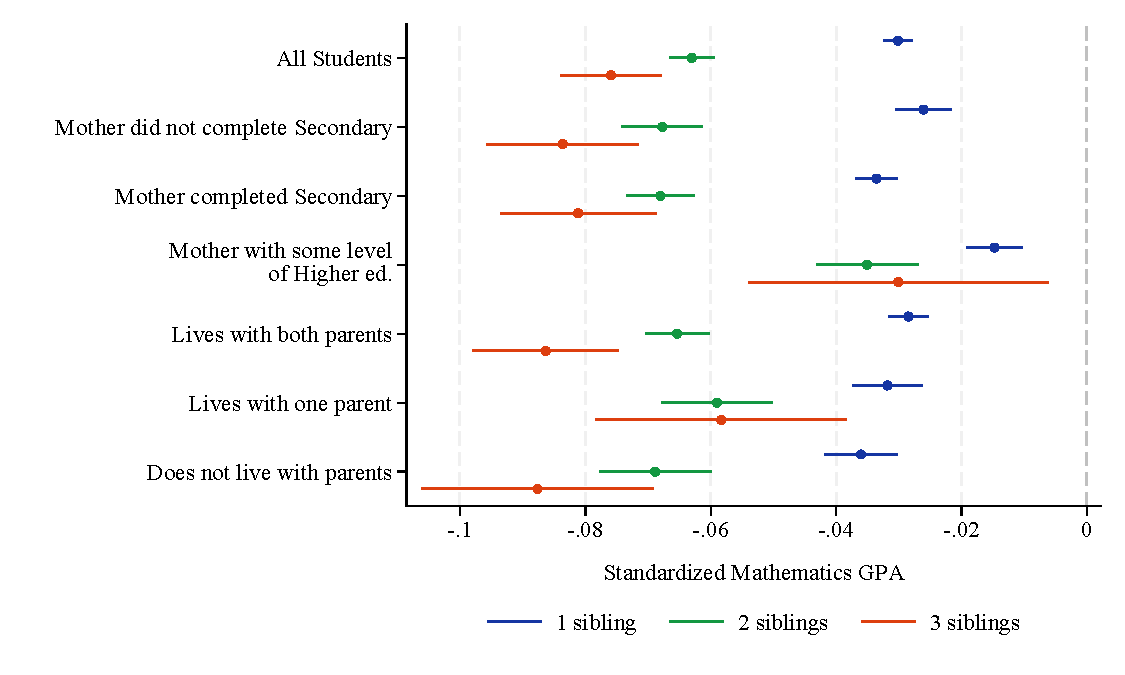
\includegraphics{./FIGURES/TWFE/covid_twfe_D_bysibs_elm_all_gpa_m_adj_Tsiblings_Soldest_4.pdf}
      }
    }

\end{transitionframe}


\begin{transitionframe}
    \label{frame:pcinternet_table}
    \frametitle{Scarce material resources: PC and Internet}
       \centering
       \resizebox{0.7\textwidth}{!}{
\makeatother
\begin{tabular}{lcccc}
\toprule
\cmidrule(lr){2-5}
& \multicolumn{4}{c}{TWFE} \\
\cmidrule(lr){2-5}
& 1-3 siblings & 1 sibling & 2 siblings & 3 siblings  \\
\cmidrule(lr){2-2} \cmidrule(lr){3-3} \cmidrule(lr){4-4} \cmidrule(lr){5-5}
& (1) & (2) & (3) & (4) \\
\bottomrule
&  &  & &  \\
\multicolumn{5}{l}{Panel D: Households with no PC or Internet} \\
Mathematics         &      -0.037***&      -0.024***&      -0.067***&      -0.089***\\
                    &     (0.005)   &     (0.005)   &     (0.006)   &     (0.010)   \\
 
&  &  & &  \\
Reading             &      -0.036***&      -0.025***&      -0.063***&      -0.083***\\
                    &     (0.005)   &     (0.005)   &     (0.006)   &     (0.010)   \\
                    &               &               &               &               \\
Observations        &     766,875   &     566,628   &     447,252   &     356,075   \\
 
&  &  & &  \\
\multicolumn{5}{l}{Panel E: Households with both PC and Internet} \\
Mathematics         &      -0.043***&      -0.024***&      -0.051***&      -0.080***\\
                    &     (0.005)   &     (0.005)   &     (0.006)   &     (0.008)   \\
 
&  &  & &  \\
Reading             &      -0.035***&      -0.018***&      -0.049***&      -0.054***\\
                    &     (0.005)   &     (0.005)   &     (0.006)   &     (0.008)   \\
                    &               &               &               &               \\
Observations        &     793,797   &     552,557   &     452,886   &     360,214   \\
 

\bottomrule
\end{tabular}
}

\end{transitionframe}

\begin{transitionframe}
    \label{frame:otherstrategies}
    \frametitle{Other potential strategies}
        \begin{itemize}
            \item Twin births: exogenous change in family size.
            \begin{itemize}
                \item Results are not significant
                \item $\approx$ 1,000 observations per grade-year of first-born with twin siblings
                \item This measures the effect of 3rd relative to 2nd child, not the effect of 2nd relative to 1st.
            \end{itemize}
            \item Same sex as instrument
            \begin{itemize}
                \item Has more power
                \item `expected change' in family size but couple with our shock may become `unexpected'
            \end{itemize}
            
        \end{itemize}
     

\end{transitionframe}



\begin{frame}
    \label{frame:byacad}
    \frametitle{By Academic achievement}
        {\resizebox{0.9\textwidth}{!}{
        %\includegraphics{./FIGURES/TWFE/covid_twfe_C_bysibs_elm_all_gpa_m_adj_Tsiblings_Soldest_4.pdf}
        \includegraphics{./FIGURES/TWFE/twfe_std_gpa_m_adj_byacad_Tsiblings_Soldest_pairall_4.pdf}
      }
    }

    \begin{flushleft}
        \hyperlink{frame:byacad_siblings}{\beamergotobutton{Results by siblings}}
    \end{flushleft}    

\end{frame}

\begin{frame}
    \label{frame:byacad_siblings}
    \frametitle{By Academic achievement}
        {\resizebox{0.9\textwidth}{!}{
        %\includegraphics{./FIGURES/TWFE/covid_twfe_C_bysibs_elm_all_gpa_m_adj_Tsiblings_Soldest_4.pdf}
        \includegraphics{./FIGURES/TWFE/twfe_std_gpa_m_adj_byacad_bysibs_Tsiblings_Soldest_pairall_4.pdf}
      }
    }

    \begin{flushleft}
        \hyperlink{frame:byacad}{\beamergotobutton{Go Back $\carriagereturn$}}
    \end{flushleft}        

\end{frame}


\begin{frame}
    \label{frame:byasp}
    \frametitle{By Education Expectations}
        {\resizebox{0.9\textwidth}{!}{
        %\includegraphics{./FIGURES/TWFE/covid_twfe_C_bysibs_elm_all_gpa_m_adj_Tsiblings_Soldest_4.pdf}
        \includegraphics{./FIGURES/TWFE/twfe_std_gpa_m_adj_byasp_Tsiblings_Soldest_pairall_4.pdf}
      }
    }

    \begin{flushleft}
        \hyperlink{frame:byasp_siblings}{\beamergotobutton{Results by siblings}}
    \end{flushleft}    

\end{frame}

\begin{frame}
    \label{frame:byasp_siblings}
    \frametitle{By Education Expectations}
        {\resizebox{0.9\textwidth}{!}{
        %\includegraphics{./FIGURES/TWFE/covid_twfe_C_bysibs_elm_all_gpa_m_adj_Tsiblings_Soldest_4.pdf}
        \includegraphics{./FIGURES/TWFE/twfe_std_gpa_m_adj_byasp_bysibs_Tsiblings_Soldest_pairall_4.pdf}
      }
    }

    \begin{flushleft}
        \hyperlink{frame:byasp}{\beamergotobutton{Go Back $\carriagereturn$}}
    \end{flushleft}        

\end{frame}


\end{document}